\documentclass[10pt,fullpage]{article}
\usepackage{epsfig,longtable}
\usepackage{times}
\usepackage{latexsym}
\usepackage{fancybox,subfigure}
\usepackage[normalem]{ulem}
\usepackage{amsmath}
\usepackage{amssymb}
\usepackage{mathrsfs}
\usepackage{verbatim}
\usepackage{appendix}

\usepackage{natbib}
\usepackage{hyperref}
\usepackage{bnf}
\bibpunct{[}{]}{;}{}{,}{,}
\bibliographystyle{plain}
%\usepackage[numbers, square]{natbib}	% citation/references
% Different font in captions
\newcommand{\captionfonts}{\small}

\setlength{\topmargin}{-0.5in}
\usepackage{latexsym}
\setlength{\columnsep}{0.5cm}
\setlength{\oddsidemargin}{-0cm}
\setlength{\evensidemargin}{-0cm}
\setlength{\textwidth}{6.8in}
\setlength{\textheight}{8.7in}

\newcommand{\remove}{}
\newcommand{\old}[1]{}
\newcommand{\match}{\stackrel{M}{=}}
\newcommand{\ncite}[1]{$^{\mbox{\tiny \citep{#1}}}$}
%\newcommand{\nncite}[1]{\citep{#1}}
\newcommand{\frags}{{\cal F}}
\newcommand{\snips}{{\cal S}}
\newcommand{\A}{{\tt A}}
\newcommand{\B}{{\tt B}}
\newcommand{\gap}{{\tt -}}
\newcommand{\ideas}{\vskip 0.6cm {\bf IDEAS:\ }}
\newcommand{\motivation}{\vskip 0.6cm {\bf MOTIVATION:\ }}
\newcommand{\mcost}[2]{#1 #2}
\newcommand{\ali}{$\mbox{ }$\hspace{0.2in}}
\newcommand{\acomment}[1]{\hspace{1in}\#{\em #1}}
\newcommand{\beqn}{\begin{equation}}
\newcommand{\eeqn}{\end{equation}}
\newcommand{\captionsize}{\footnotesize}
\newcommand{\LtoN}[1]{\parallel #1 \parallel_{2}}
\newcommand{\mecca}{HapCUT$\:$}
%%%%%%%%%%%%%% FIGURE within a box
\newenvironment{boxfig}[1]{\fbox{\begin{minipage}{\linewidth}
                        \vspace{1em}
                        \makebox[0.025\linewidth]{}
                        \begin{minipage}{0.95\linewidth}
                        #1
\end{minipage}
                        \end{minipage}}}
                                                                                                                                                                            
\def\ensuretext{\textrm}
\newcommand{\Reads}{\ensuretext{{\sc Reads}}}
\newcommand{\AlignStr}{\ensuretext{{\sc AlignStr}}}
\newcommand{\Intervals}{\ensuretext{{\sc Intervals}}}
\newcommand{\Strand}{\ensuretext{{\sc Strand}}}
\newcommand{\Partner}{\ensuretext{{\sc Partner}}}
\newcommand{\MST}{\ensuremath{\mathit{MST}}}
\newcommand{\dist}{\ensuremath{\mathit{dist}}}
\newcommand{\TG}[2]{\ensuremath{\mathit{#1}^{(#2)}}}
\newcommand{\CC}{\ensuremath{\mathcal{CC}}}
\newcommand{\psubs}{\stackrel{\subset}{+}}
\newcommand{\rs}{\ensuremath{\mathit{R_s}}}
\newcommand{\MEC}{\ensuremath{\mathit{MEC}}}
\newcommand{\Prob}{\ensuremath{\mbox{Pr}}}
\newcommand{\fref}[1]{\mbox{Figure~\ref{#1}}}
\newcommand{\secref}[1]{\mbox{Section~\ref{#1}}}
\newcommand{\para}[1]{\vspace{2pt}\noindent\mbox{{\bf #1:} }}
\newcommand{\slimfast}{{\sc SlimGene}}

%%%%%%%%%%%%%%%%%%%%%%%%%%%%%%%%
% GenomeQL syntax
%%%%%%%%%%%%%%%%%%%%%%%%%%%%%%%%%%%
\newcommand{\MapRel}{\ensuremath{\:\overline{\bowtie}\:}}
%\newcommand{\MapRel}{\ensuremath{\stackrel{\bowtie}{\llcorner\lrcorner}}}
\newcommand{\NatJoin}{\ensuremath{{\bowtie}}}
%\newcommand{\MapRel}{\ensuremath{\bowtie_M}}
\newcommand{\Project}[1]{\ensuremath{\Pi_{#1}}}
\newcommand{\ProjectInterval}[1]{\ensuremath{\Pi^i_{#1}}}
\newcommand{\Select}[1]{\ensuremath{{\displaystyle \sigma_{#1}}}}

\newcommand{\gqlSelect}{{\sc select}}
\newcommand{\gqlFrom}{{\sc from}}
\newcommand{\gqlWhere}{{\sc where}}
\newcommand{\gqlAnd}{{\sc and}}
\newcommand{\gqlAvg}{{\sc avg}}
\newcommand{\gqlMin}{{\sc min}}
\newcommand{\gqlMax}{{\sc max}}
\newcommand{\gqlIn}{{\sc in}}
\newcommand{\gqlAbs}{{\sc abs}}
\newcommand{\gqlCount}{{\sc count}}
\newcommand{\gqlGroupby}{{\sc groupby}}
\newcommand{\gqlIntersects}{{\sc intersect}}
\newcommand{\gqlMapjoin}{{\sc mapjoin}}
\newcommand{\gqlProjectInterval}{\gqlSelect\ {\sc merged}}
\usepackage{latexsym}

%%%%%%%%%%%%%%%%%%%%%%%%%%%%%  THEOREM-LIKE ENVIRONMENTS
                                                                                                                                                                            
\newtheorem{THEOREM}{{\bf  Theorem}}
\newenvironment{theorem}{\begin{THEOREM} \hspace{-.85em}  {\bf :} }%
                        {\end{THEOREM}}
\newtheorem{LEMMA}[THEOREM]{Lemma}
\newenvironment{lemma}{\begin{LEMMA} \hspace{-.85em} {\bf :} }%
                      {\end{LEMMA}}
\newtheorem{COROLLARY}[THEOREM]{Corollary}
\newenvironment{corollary}{\begin{COROLLARY} \hspace{-.85em} {\bf :} }%
                          {\end{COROLLARY}}
\newtheorem{PROPOSITION}[THEOREM]{Proposition}
\newenvironment{proposition}{\begin{PROPOSITION} \hspace{-.85em} {\bf :} }%
                            {\end{PROPOSITION}}
\newtheorem{CLAIM}[THEOREM]{Claim}
\newenvironment{claim}{\begin{CLAIM} \hspace{-.85em} {\bf :} }%
                      {\end{CLAIM}}
\newtheorem{OBSERVATION}[THEOREM]{Observation}
\newenvironment{Observation}{\begin{OBSERVATION} \hspace{-.85em} {\bf :} }%
                      {\end{OBSERVATION}}
\newtheorem{DEFINITION}{Definition}
\newenvironment{definition}{\begin{DEFINITION} \hspace{-.85em} {\bf :} }%
                           {\end{DEFINITION}}
\newcommand{\QED}{\hfill$\clubsuit$ \vskip 0.1cm}
\newenvironment{proof}{\noindent {\bf Proof:} \hspace{.677em}}{\QED}
\newenvironment{packed_enum}{
\begin{enumerate}
  \setlength{\itemsep}{1pt}
  \setlength{\parskip}{0pt}
  \setlength{\parsep}{0pt}
}{\end{enumerate}}
\newenvironment{packed_itemize}{
\begin{itemize}
  \setlength{\itemsep}{1pt}
  \setlength{\parskip}{0pt}
  \setlength{\parsep}{0pt}
}{\end{itemize}}

% define the title
\author{Vineet Bafna\thanks{Computer Science and Engineering, UC San Diego}\and Alin Deutsch$^*$\and Andrew Heiberg$^*$\and Christos Kozanitis$^*$\and Lucila Ohno-Machado\thanks{Division of Medical Informatics, UC San Diego}\and George Varghese$^*$}
\title{Abstractions for Genomics: Or, which way to the Genomic Information Age?}



% packages
\usepackage{graphicx}
%\usepackage{subfig}

%document
\begin{document}
\maketitle

\begin{abstract}
  With DNA full sequencing costs dropping below \$$1,000$, two major
  application drivers are: finding the genetic basis for disease (via
  Genome Wide Association Studies), and personalized medicine
  (tailoring treatments to genetic makeup as in cancer genomics).
  While hardware costs are falling, software costs are a major
  obstacle to both discovery and personalized medicine.  In this
  paper, we propose attacking this obstacle via the use of a
  hierarchical set of abstractions (akin to Internet layers) for
  genome processing.  While interface formats exist for mapped files
  (BAM) and variant formats (VCF), we propose a new separation of
  variant calling into a deterministic evidence layer that is queried
  by a probabilistic inference layer via a proposed Genome Query
  Language.  GQL allows inference engines to efficiently sift only the
  relevant evidence (e.g., the READs that flank a SNP site) from raw
  genomic data.  

%  We argue that the current lack of modularity is largely a remnant of
%  scarcity thinking from an era when sequencing was expensive and
%  hence every last drop of inference had to be squeezed from limited
%  data.

  We describe a set of exemplar queries ranging from SNP calling to
  phasing based on input from sequencing companies and show how
  evidence for these queries can be concisely captured using GQL.
  Discovery is modeled as finding the variants common to a given
  phenotype, and personalized medicine as the dual problem of finding
  the phenotypes corresponding to individual variations, from a
  database of complete individual genome sequences.  We suggest that
  the standard implementation of GQL using relational database tables
  with billions of rows for each genomic location will not scale to a
  single human; instead, we introduce efficient indices based on
  compressed strength vectors to scale to large populations.  We
  outline several benefits to separating evidence from inference
  including the ability to reuse genomic data across studies, the
  ability to logically assemble case-control cohorts, and the ability
  to rapidly change queries without customized programming. Finally,
  GQL allows us to move away from deep analysis of individual genomes
  towards group inference on large populations.  Our paper is written
  for computer scientists: it starts with a model of genetic
  processing assuming no prior knowledge, and ends with a set of
  challenges in computer systems, security, information retrieval,
  inference, and databases.
\end{abstract}

\section{Introduction: Universal sequencing: opportunities and problems}

We are a product of ``nature and nurture''. By this, we mean that our
\emph{phenotype} (the composite of all outward, measurable,
characteristics including our health parameters) is a function of two
things: our \emph{genotype} (the DNA program inside all cells), and
the environment (all the inputs to a human including food and
medicine).  For a computer scientist, a useful analogy can be drawn
from how the output of a program (e.g., an Internet search engine) is
a function of both the program and the input (keywords typed by
user). Specifically, using the same input with a different program
(e.g. Google search vs. Bing) is likely to result in a different
output.

In this analogy, the role of the medical professional is to provide
information that is either ``diagnostic'' (i.e. is there a bug in the
program based on observed output?), ``prognostic'' (e.g., can we
predict the output/outcome, given specific inputs such as diet?), or
``therapeutic'' (e.g., can any specific input such as a drug lead to
the desired output). Also, the Electronic Medical Record (EMR) of a
patient can be described as an archive of previously acquired inputs
and outputs.  While this is a useful analogy, there are subtle
differences.  Unlike computers, the human hardware (the body) itself
is the output of programmed instructions and previously received
input; thus, each program runs on unique and constantly changing
hardware.  Additionally, the program itself changes over the course of
the lifetime of the individual due to acquired mutations in the DNA,
but we will not discuss this here.

Unlike computers, the human ``program'' was largely hidden away with
only the hardware visible. As a consequence, medicine has
traditionally been ``not-personalized'' with doctors providing
treatments based on comparisons of the patient's phenotype (symptoms)
against empirical observations of outputs from a large number of
individuals.  However, there is some customization based on
observation of phenotypes from `similar' individuals based coarse
classes such as `race'.  All of this changed with the sequencing of
the human genome in early 2000, and the subsequent drop in costs from
hundreds of millions of dollars down to \$1000 on small desktop
sequencing machines. The ability to cheaply read the program of each
human underlies the great promise of \emph{personalized medicine}---
treatments based on symptoms and the patient's distinctive program
(i.e., DNA).

We frame this point with a classic example. The blood-thinner drug,
Warfarin, has seen myriad previous uses, including as rat-poison
during World War I~\citep{Thomson1991}, to treat
Eisenhower~\citep{Link1959}, and allegedly to poison
Stalin~\citep{Brent2003}. It is now a widely prescribed anti-coagulant
therapy against blood clot formation. The dosage is critical: too
high, and the patient can bleed to death; too low and the drug may not
prevent life-threatening blood-clots. Often, the right dosage is
established through multiple visits to the clinic, and regular
testing. However, recent reports~\citep{Schwarz2008} suggest that
knowledge of the patient's genetic program can help establish the
right dosage. The approach to discover the genetic association of drug
response is standard in the field, and outlined below.
\begin{packed_itemize}
  \item Collect a sample of affected, and `genetically matched' control individuals.
  \item Sample the DNA and catalog variations in the populations.
  \item Identify and  report variations that co-segregate (i.e., correlate) with the affected/control status of the individual.
  \item Follow up on the genetic basis of the correlation through
    expensive follow-up studies and experiments in animal models
    and clinical trials. Transfer knowledge to the clinic.
\end{packed_itemize}
We dub this sequence the {\em discovery} workflow. Much of the
discovery workflow is carried out by trained researchers, and
subsequently adapted for clinical use. Even with its successes, the
discovery approach has some problems.  First, such studies are
resource intensive and rely on the researcher's ability to identify
and sequence large cohorts of individuals with and without a
disease. Second, it is unclear how to apply the study results to a
specific individual, especially one that is genetically different from
the investigated cohort.  Finally, a specific study often looks at
only a small subset of variants, and the entire data is then dumped
into archives. Significant computational burden must be expended to
dig out data from a previous study, and a lot of care needs to be
exercised in using the data (See, for example,``\$100 Genome with a
100,000 dollar analysis''-Stanford Medicine, 2010) and to make
inferences across datasets from different labs.

We contrast the discovery work flow with \emph{personalized
  medicine}. Here, a physician treating individual $A$ may query a
database either for: treatments suitable for patients who have genetic
variations similar to those of $A$; or query for patients genetically
similar to $A$ for treatments and dosages that worked well for these
patients. 

Indeed, the notion of computational tools enabling personalized
medicine is well received. Many groups have proposed specialized
databases for cancer genomes which are marked by an excess of somatic
(non-inherited) mutations\cite{Patterson2011,Haussler2011}. As these
databases come online and more details become available, we can
compare the different visions. Here, we take a more general viewpoint,
arguably allowing for broader access to genomic information, and
enabling both discovery and personalized medicine.

Specifically, we suggest a shift in perspective. Instead of sequencing
small cohorts on a need-to basis, we assume that \emph{each}
individual is sequenced at birth, and her personal genome is an
integral part of her EMR (medical record), and available to be queried
by trained researchers and medical personnel. This scenario is
realistic considering the rapid drop in sequencing costs.

In the example of choosing Warfarin dosage for a patient, the medical
team might do the following: (a) identify a collection of individuals
genetically similar to the patient and on a warfarin regimen; (b)
query their genomes and EMRs for genetic variation in candidate genes
and warfarin dosage, respectively; and, (c) choose the appropriate
dosage based on the patient's specific genetic program. The ability to
logically select from a very large database of individuals using the
phenotype as a key removes the first problem described with the
discovery workflow.  Using genetic variations specific to an
individual $A$ as a key to return treatments (that work well for such
variations) addresses the second problem.  Finally, if the EMRs and
genomic information is maintained in a uniform manner, and the
accompanying software system has good abstractions for querying across
various experiments, then the third problem (computational burden to
reuse data) is also greatly eased.

Thus our major thesis is that the simple shift in perspective to
assuming that the genome sequence of all individuals is available to
be queried (see Figure~\ref{fig:fig1}) helps {\bf 1)} decrease bias
for discovery and {\bf 2)} enables personalized medicine.  Realizing
this requires the ability to provide suitable abstractions that are
flexible enough for stakeholders such as experiments and physicians,
and yet easy to use.  Our paper focuses on proposing new abstractions
for genomics along with efficient implementations.  In computer
science, key abstractions such as virtual memory and relational data
models have vastly improved productivity and reduced software costs to
keep pace with cheap VLSI hardware: our central thesis is that the
same is required for genomics.



\begin{figure}[htbp]
  \centering
  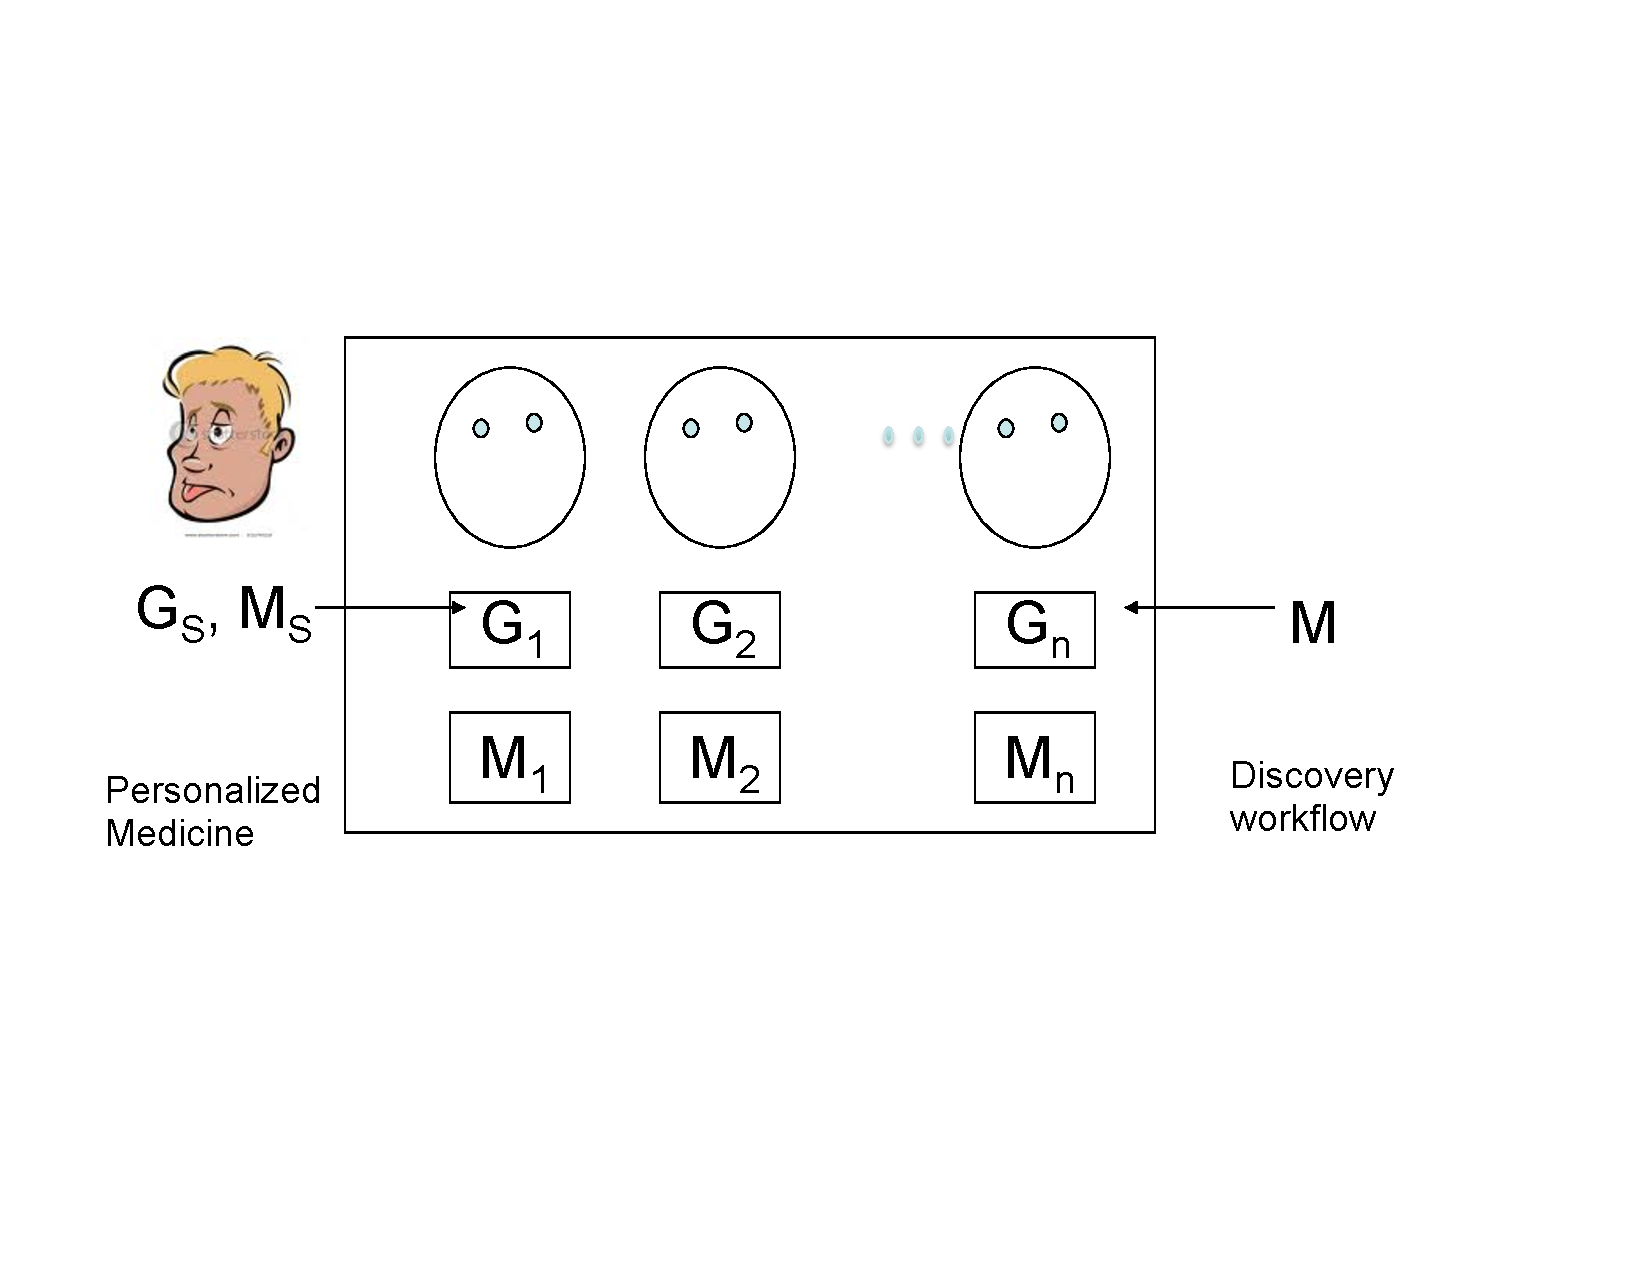
\includegraphics[trim = 15mm 70mm 20mm 50mm, clip, width=5in]{fig/personalizedmedicine.pdf}
  \caption{{\bf Genome Sequencing and personalized medicine}. We
    consider the scenario where every individual is sequenced at
    birth. The Discovery workflow starts with logical selection of a
    subset of individuals with a specific phenotype (e.g., disease)
    and another without the phenotype, and then identifying genetic
    determinants for the phenotype. By contrast, Personalized medicine
    can be seen as the task of retrieving the medical records and
    genotypes of all patients genetically similar to a sick patient
    S.}
  \label{fig:fig1}
\end{figure}

Further, computer systems designers often benefit from systems
thinking: making tradeoffs at the component level for overall
benefits, and leveraging technology trends. We will argue that system
thinking is badly required in genomics because genomic processing was
invented in an era of scarcity, where genomes were scarce and
sequencing was expensive; the time has come to rethink these
assumptions.  This article is written so that computer scientists ---
not just bioinformaticians who have already contributed so much, but
computer scientists of every ilk and especially computer systems
researchers --- can engage with biologists and doctors in an essential
endeavor to improve the health of the planet.

We note upfront that new genomic technologies are also helpful in
sampling the dynamic states of the cell. For example, transcript
sequencing technologies (e.g. RNAseq) provide a direct look at which
genes might be activated, or repressed in specific contexts. Likewise,
other technologies probe the cell from a systems biology viewpoint
decoding networks of interacting proteins, RNA, and DNA (See
Section~\ref{sec:genetics}) for definitions. However, we limit the
scope of this article to genomic databases, and the study of how
inherited variations. Moreover, we do take a more abstract treatment
of current technologies, and do not discuss specific technologies
(e.g. Pacific Biosciences strobe sequencing, LifeTech color space
encoding, single molecule sequencing) and other technical issues.

\old{
\begin{figure}[h!]
  \centering
  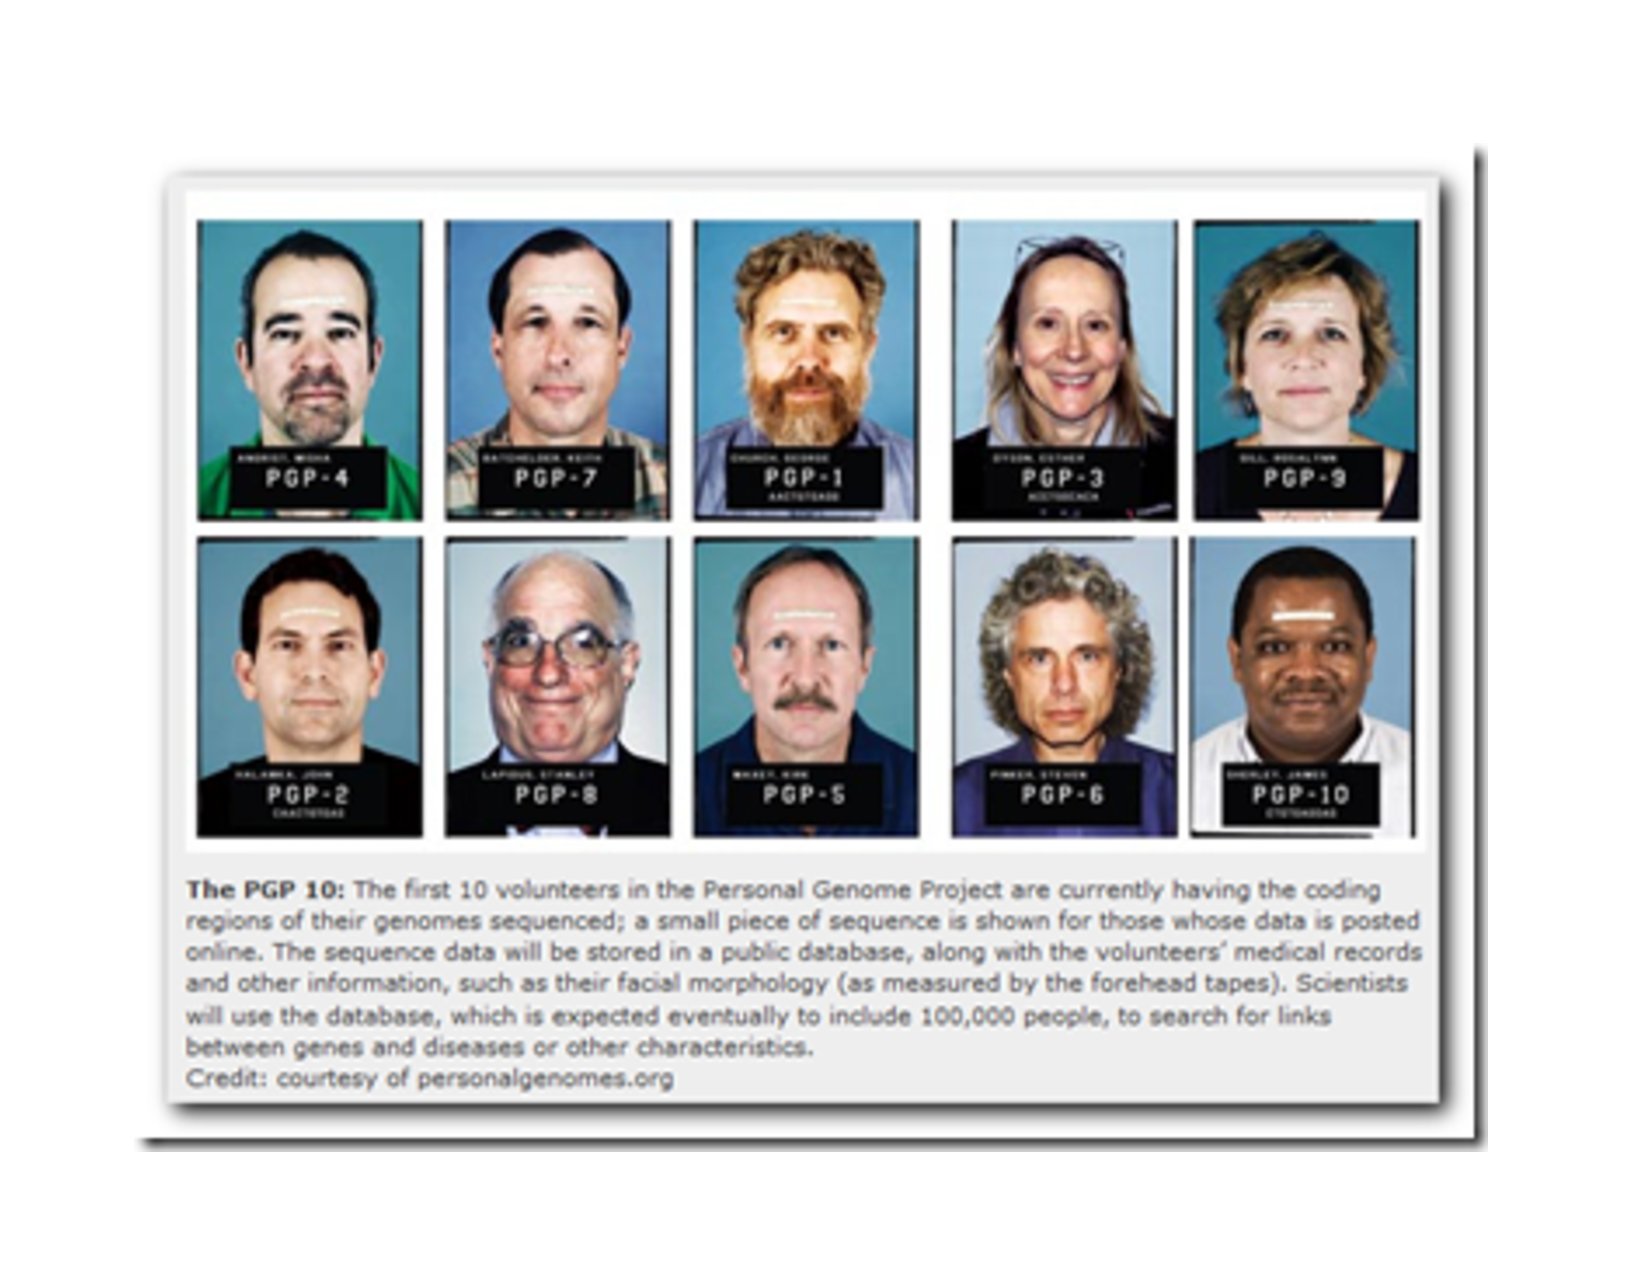
\includegraphics[trim = 0mm 20mm 0mm 20mm,clip, width=6in]{fig/PMD.pdf}
  \caption{An initial version of the Personal Medicine Database, the
    Personal Genome Project.  While the project is filling the
    database, it has not developed query abstractions. {\bf XXX we
      will need permission for this figure reproduction.}}
  \label{fig:PMD}
\end{figure}
}
                    
To begin the conversation, we start by describing basic genetics using
programming metaphors and introduce some of the terminology
(Section~\ref{sec:genetics}). Section~\ref{sec:trends} describes
recent developments in sequencing, and continuing trends for the near
future. With these preliminaries, we offer some advanced examples in
Section~\ref{sec:usecases} describing the state-of-the-art of genome
querying, and motivating the abstractions for genome queries. Our
vision for a vast genomic database built in layers is described in
Section~\ref{sec:vision}--- the key idea here is the separation of 
`evidence' and `inference'.  In Section~\ref{sec:gqa}, we propose
an algebra for specifying genome queries, extending ideas from
Databases, String matching algorithms, and Computer Systems. We end in
Section~\ref{sec:futuredirections}) by outlining research directions
for other areas of computer science to further this agenda.

\section{Genetics for Computer Scientists}
\label{sec:genetics}
The following is a quick introduction to the relevant biology and
terminology used in the sequel for computer scientists.  The reader is
urged to consult a standard reference for
details (~\citep{Alberts2007}).

All living creatures consist of cells; each cell can be considered to
be a computer running a program which is its DNA.  Humans are {\em
  diploid} --- there are two programs controlling each cell, one
inherited from the father and one from the mother.  Further, each
program is broken up into $23$ ``modules'' called chromosomes and
within each chromosome are sparsely scattered small functional blocks
called genes. The module pairs from the father and mother are called
homologous chromosomes and each human has a pair of genes from each
parent.  Each program uses a 4-character alphabet of bases (A,C,G,T)
and is around 3 billion bases long.

Much of the `hardware' of the computer consists of cellular organelles
and proteins--- the cellular machinery. Proteins are folded sequence
of amino acids, and perform specific cellular functions such as
catalyzing metabolic reactions, transducing signals, and so on. The
gene contains the `code' for manufacturing proteins. Each gene
executes in one of many `ribosomes' (analogous to a CPU).  Information
travels from the nucleus (where the packaged DNA resides) to the
ribosome via a `messenger' molecule (mRNA) that is essentially a copy
of the coding DNA. The ribosome `reads' the code 3 bases (one codon)
at a time. Each codon is analogous to an OpCode instructing the
ribosome to attach a specific amino acid to the protein sequence being
constructed. Thus, the DNA program can provide instructions for making
the hardware which in turn performs all cellular functions.

\begin{figure}[tbph]
  \centering
  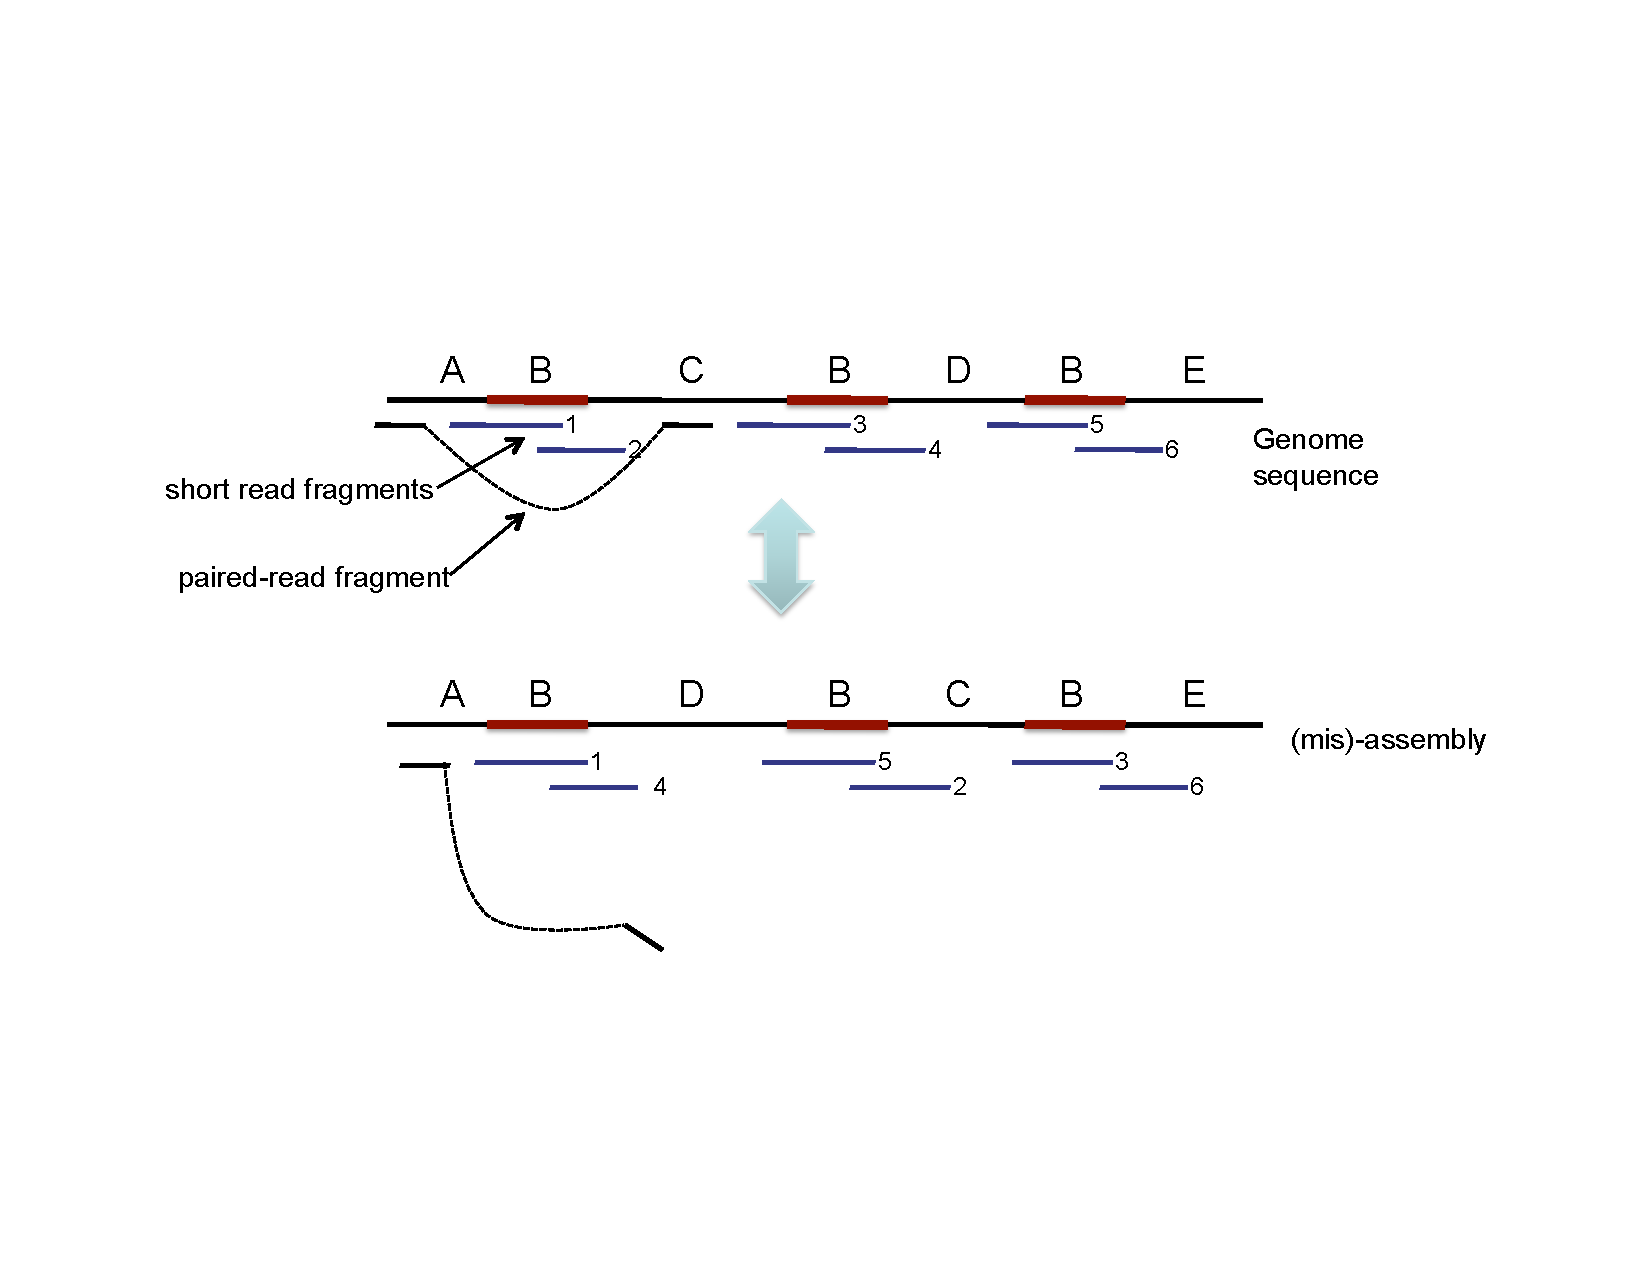
\includegraphics[trim = 20mm 50mm 20mm 60mm, clip,width= 4.5in]{fig/repeat_assembly.pdf}
  \caption{{\bf Repetitive nature of genomic sequence and its
      assembly}. $40\%$ of the human genomic sequence is made up of
    repetitive sequence. In this illustration, region B appears in 3
    copies while regions A,C,D,E are unique. Assembly is confounded if
    the length of repetitive regions exceeds the length of reads. In
    this case the overlaps in short reads numbered 1 through 6 are
    equally consistent with two possible architectures. However, a
    single paired-end read from a clone that spans a repeat sequence
    sampling unique regions A and C, is consistent with the true
    sequence, but not with the alternative sequence (the two ends are
    mapped far apart).}
  \label{fig:repeatassembly}
\end{figure}

A change (\emph{mutation}) in the DNA can change the amino-acid, and
correspondingly, the cellular machinery resulting in a different
phenotype (output). In the Mendelian paradigm, each of the two
homologous copies of the gene controls one {\em phenotypic trait}
(e.g., ability to clot blood). A mutation in one gene might impact the
phenotype strongly (\emph{dominant}), not at all (\emph{recessive
  mutation}) or somewhere in between. In fact, most phenotypes are
\emph{complex}--controlled by the paired copies of multiple
genes. Nevertheless, DNA controls traits so even the simplest queries
on DNA are useful --- e.g., {\em Compared to a `normal' individual,
  are there parts of the patient's DNA program that have mutated}.

Advancements in sequencing has made it possible to cheaply scan an
individuals genetic program for mutations (or, \emph{variations}).
First, a physical process is used to randomly shear genomic DNA into
small \emph{inserts} of size $500$-$10000$bp. The sequencing machines
deciphers the DNA from small \emph{fragments, or reads} (length
$L\simeq 100$bp) at one or both ends of the inserts.  Thus, the
genomic information is presented as a collection of small strings over
A,C,G,T, sampled from a random location on a (maternal or paternal)
chromosome. Rapidly changing technologies change the throughput of
sequence, insert-lengths, and read lengths, and we will discuss these
parameters in the next section.

It is natural to assume that these fragments will be assembled like a
giant jigsaw puzzle.  However, this is complex and expensive because
of the large amounts of repetitive portions in human genomes
(Figure~\ref{fig:repeatassembly}).

\paragraph{Mapping, and Variation:}
An alternative to assembly is to \emph{align}, or \emph{map} the
fragments of a sampled genome (the \emph{donor/patient genome}) to a
reference human genome, such as a current version of a reference human
genome assembly~\citep{Celera,Genome2004}. Note that the assembly is a
single (haploid) copy of each chromosome sampled from multiple
individuals. Mapping involves finding a location on the reference
where the genomic substring matches the query fragment up to a small
number of errors. The errors might be sequencing errors or true
variations in the query, relative to the reference. In case of
multiple matches, the `best' match is returned, sometimes with some
alternatives. Mapping new patient genomes works because string search
is cheaper than assembly and any pair of human genomes is identical to
1 in $1000$ locations.

A true deviation in the sequence of the donor, relative to the
reference is called a {\em variation}.  The simplest variation is a
\emph{SNV} (single nucleotide variation). As the donor genome consists
of two copies, we can be more precise in cataloging variations. A
\emph{homozygous} variation occurs in both copies; if it occurs in
only one copy, it is said to be {\em heterozygous}. The specific value
of the variant is called an \emph{allele}. For example, suppose that
the DNA at homologous chromosomes of individual $A$ compared to the
reference is as follows
\[
\begin{array}{cl}
\cdots ATG\cdots GAGTA\cdots & \mbox {Reference Assembly}\\
\cdots ACG\cdots GAGTA\cdots & \mbox {Maternal chromosome 1}\\
\cdots ATG\cdots GAGCA\cdots & \mbox{ Paternal chromosome} 
\end{array}
\]
Then, individual $A$ is bi-allelic, or heterozygous at the 2 SNV
sites, has the \emph{genotype} $\cdots C/T\cdots C/T\cdots$, and the
genotypes are resolved into two \emph{haplotypes} $\cdots C\cdots
T\cdots,\cdots T\cdots C\cdots$.


Sites containing SNVs that are prevalent in a population demarcate
chromosomal positions as varying, or polymorphic. Consequently, these
locations are called \emph{SNPs} (Single Nucleotide Polymorphisms). In
discovery workflows, we test populations to see if the occurrence of
variation correlates or \emph{associates} with the phenotype status of
the individual.

All of this refers to simple variation involving one, or a small
number of changes at a location. By contrast, we also have
\emph{structural variations} in which large (one kbp to several
million bases) genomic fragments are deleted, inserted, translocated,
duplicated, or inverted, relative to the
reference~\citep{Tuzun05}. The impact of these changes on the
phenotype are only now beginning to be appreciated~\citep{Lupski02}.


\section{Trends in genome sequence technology}
\label{sec:trends}
The following trends are relevant to the system design of genomic software:

\begin{itemize}
\item {\em Costs are reducing:} The Human genome project required over
  $22500$ hours of sequencing, and cost $\sim \$100M$. Human
  re-sequencing costs for a redundant ($15\times$) coverage are now
  under \$5K, and projected to go below \$1K very soon. This implies
  that universal sequencing may soon be realizable, and that complex
  inference techniques on small populations may be replaceable by
  simpler inference techniques on large populations.  Further, it
  implies that archival and analysis, not sequencing, will dominate
  cost.

\item {\em Read lengths will continue to be small:} The Sanger
  sequencing technology used for the human genome project has long
  Read lengths and could achieve $100\times$ multiplexing on
  capillaries with sequence lengths between $700$ - $1000$, to get
  $100$kbp in $3$ hours per machine.  However, capillary sequencing
  has largely ceded ground to new sequencing technologies that
  sacrifice length and sequence quality to massive
  parallelism and high throughput (achieving close to $600$Gbp per
  machine per 11 day run)~\citep{HiSeq2000}.  While newer,
  `single-molecule' sequencing technologies promise to deliver longer
  read lengths at the expense of quality and
  throughput~\citep{PacBioRS}, it seems likely that in the near
  future, individuals will be sampled using relatively short read
  fragments ($<10000$bp).  This implies that useful abstractions must
  consider fragments and mapping as first-class entities.

\item {\em Assembly continues to be hard and paired end sequencing will be useful:}  Repetitive regions cover
$\sim 40\%$ of the human genome. If the read-length is shorter than
the length of repetitive sequence, the genome cannot be assembled
uniquely.   Longer reads or reads sequenced from ends of long clones (paired end 
reads) are necessary to resolve repeats
and assemble sequences \emph {de novo}. Therefore, current emphasis is
on \emph{re-sequencing} applications in which the sequenced reads are
mapped to a standard human reference to identify variations, and
correlate these variations against phenotypes. Even with improving
technologies as well as assembly algorithms, it is likely that
scientists will want to retain, and query the short read data used to
generate the assembled sequence.  Once again, this implies that fragments
and reads (and paired-end reads) must be first class entities. 

\item {\em Computer System Costs will soon dominate:} Some studies
\cite{Stein2010, Pennisi2011}
  have shown that the costs of disk storage for genomes is now greater
  than the costs of sequencing and the cost of sequencing is dropping
  faster than the cost of disk storage.  Disk storage is only a small
  portion of overall system costs.  This implies the need for good
  abstractions that can reduce system costs, potentially sacrificing
  information quality for modularity and making up for this loss by
  marshalling large quantities of data.
\end{itemize}

Therefore, we start with the premise that the genome sequence of an
individual will continue to be in the form of fragments (possibly with
an assembly) in the near future. We start by presenting some
biologically inspired queries. The main point to note here is that
there are many methods to make biological discoveries from sequence
data, and no consensus on the best method.  Abstractions must be
flexible to handle the variety of methods some of which are surveyed
in the next section.

\section{Variation Calling Today}
\label{sec:usecases}
The key to efficiency in genomics is the premise that an individual's
genetic record can be summarized succinctly by a much smaller list of
individual genetic variations.  While we develop this premise further
in our layering proposal (Figure~\ref{fig:abstraction}a)), we use this
section to provide the reader with some intuition in how variants are
called {\em today}.  The expert should skip this section and proceed
to our layering proposal. We start with querying for Single Nucleotide
Variations (SNVs) in the donor genome, the simplest form of variation.

\subsection{Calling SNVs}
Figure~\ref{fig:variationevidence} shows how a mutation may be called.
Consider the reference allele {\em C}. We see two copies of the donor
genome with a {\em G} allele, and some copies with {\em C}, indicating
a heterozygous SNV.If the variation is homozygous, we expect all
overlapping READs to have a {\em G} in that position. Even this simple
call can be confounded. First, some of the reads may have been mapped
to the wrong place on the reference; such as the top donor read in the
figure. The G/T mutation may not be correct and the alignment of the
incorrectly mapped read might present many variations. Even if the
READ is mapped correctly, sequencing errors can present themselves as
heterozygous mutations.

Thus, mutation callers use various statistical methods informed by
mapping quality (e.g., the number of potential places in the genome a
read can map to) of the read, the quality score of a base call, and
the distribution of bases or alleles in the READs for that location.
Some mutation callers even use evidence based on the surrounding
locations (e.g., is there an excess of insertion/deletion events
nearby suggesting problems in alignment). The decision itself could be
based on frequentist, Bayesian inference, or other machine learning
techniques.  While SNP callers use various inference techniques, they
all use the same evidence: the set of reads overlapping the location
of the SNP in question.
 
\subsection{Calling Structural Variations-- Deletions, Inversions etc}
In addition to small nucleotide changes, larger structural variations
involving insertion, deletion, and translocation of large genomic
regions also form an important source of genomic variation. Detection
and characterization of large Structural Variations (SVs) is a
challenging research problem. We consider the example of deletions in
the donor genome (a large segment of DNA is deleted, relative to the
reference). If both copies of the donor genome are deleted, the
deletion is said to be {\em homozygous}; otherwise, it is a {\em
  heterozygous} deletion. Deletions can be detected using a number of
techniques:

\begin{figure}[htbp]
  \centering
  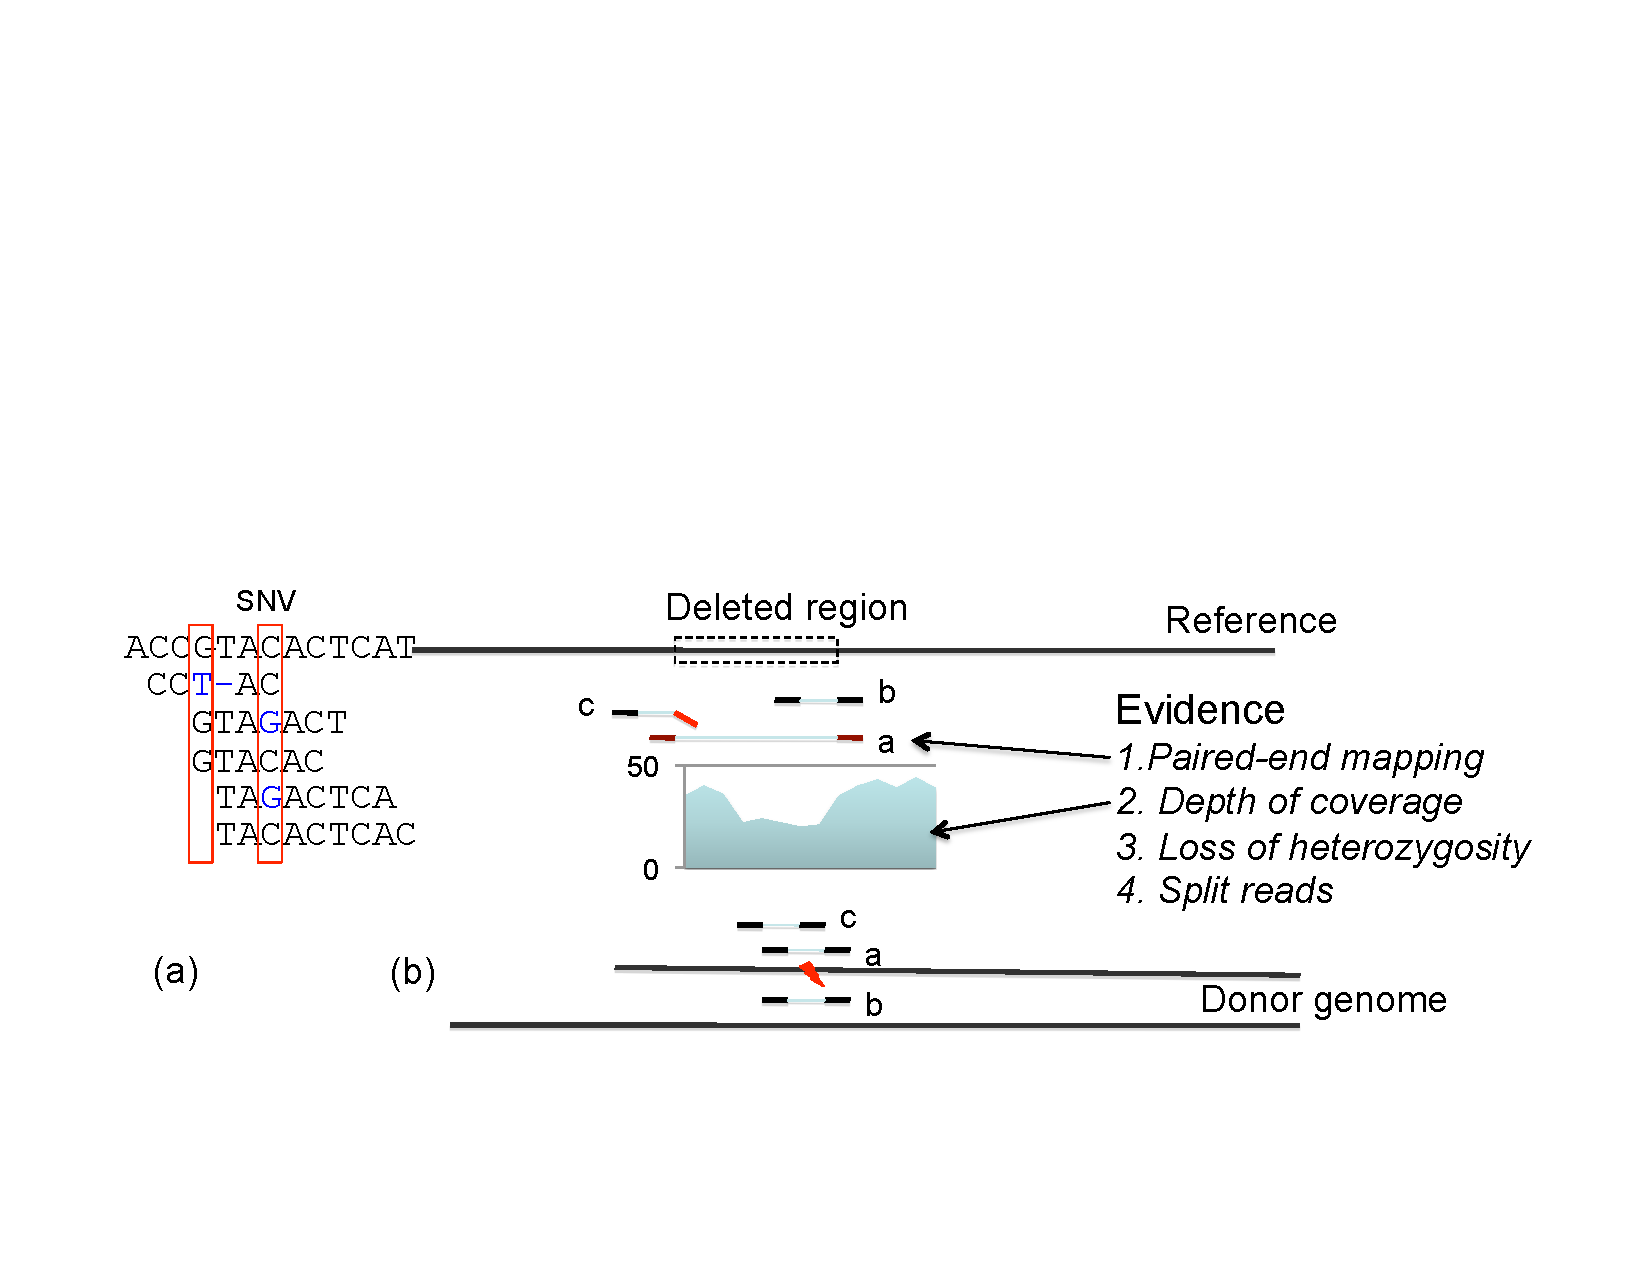
\includegraphics[trim = 5mm 30mm 5mm 50mm, clip, width=5in]{fig/deletion_and_SNV_evidence.pdf}
  \caption{{\bf Evidence for variation in the donor}. (a) The evidence
    for SNVs is provided by aligning donor reads against the reference
    sequence. The G/T variation might be a sequencing error as the
    variant reads maps with two many errors. However, the G/C
    variation appears to be a true SNV. (b) Paired-end sequencing and
    mapping provides evidence for deletion in the genome. The dotted
    rectangle demarcates the region in the reference deleted in
    exactly one of the two donor chromosomes. Read `a' samples the
    region around the deletion, and maps `discordantly' in the
    reference; read `b' maps concordantly, but with coverage about
    half of neighboring regions; read 'c' is sampled from the
    breakpoint and can map only at one end. }
  \label{fig:variationevidence}
\end{figure}
\paragraph{Paired-end mapping:} In Paired-end sequencing, both ends of
large genomic fragments (sampled randomly from the donor genome) are
sequenced. These genomic fragments have been size-selected to be
tightly distributed around an insert length $L$. In a normal
situation, when the paired-ends are mapped back to the reference
(paired-end mapping), the two ends map around $L$ base-pairs apart. If
however, they end up mapping much further apart than expected
(\emph{length-discordance}), we can infer a deletion in the donor
relative to the reference. For example, $L\simeq 500$bp is a typical
insert length. If the two ends map about 700bp apart, that may be
consistent with natural variation in insert size. However, if they map
$10$kbp apart, we can infer a deletion of $9.5$kbp. If the deletion is
heterozygous, we should see a mix of concordant and discordant reads
at the breakpoints of the deletion. 

\paragraph{Depth of coverage:}
Here, ``depth'' at a position refers to the count of reads mapped to
the position.  As the fragmentation is considered random, the genome
is uniformly covered by read fragments. Deleted regions of the donor
chromosome will have reduced coverage (roughly half for heterozygous
deletions and zero for homozygous ones). Thus the depth of coverage is
a clue to identifying deletions.

\paragraph{Loss of heterozygosity:} Consider the SNV locations on the
donor genome. At any specific polymorphic location with major allele
frequency of $p$ in a population, the Hardy-Weinberg principle
suggests that a diploid individual (with 2 copies) is homozygous with
probability $p^2+(1-p)^2$, and heterozygous
otherwise\cite{HartlClark}. Clearly, while sampling multiple
polymorphic sites, we expect a mix of heterozygous sites. When a
deletion occurs, the single chromosome being sampled displays a loss
of heterozygosity.

\paragraph{Single end mapped, and split-reads:} When a read maps to
the breakpoint of the deletion on the donor, it cannot be mapped back
to the reference. In the case of a `clean' deletion, the prefix and
suffix of the fragment could be mapped separately, and such
split-reads are indicative of deletion events. Often, the occurrence
of breakpoints in repeat regions, and the presence of non-templated
insertions makes this harder, but split reads are still useful clues
for small deletion events.

Even, within these four categories, a number of design decisions are
made by individual tools to improve the sensitivity, and specificity
of detection. For example, the counts in a ``depth of coverage''
calculations must be sensitive to repeats and other natural variation
in read coverage; the natural length variation in insert size must be
accounted for in paired-end mapping; conflicting evidence from these
orthogonal clues must be reconciled, as also read quality, and mapping
quality must be accounted for. Thus, the prediction of deletion and
other SVs remains a challenging research problem, much like the
prediction of SNVs. In these scenarios, the problem of high throughput
querying of genomes remains challenging.

We also note that genomics today is dominated by what we call {\em
  scarcity thinking}.  Three examples of scarcity thinking follow.
First, a human genome is stored using 250 Gbytes of storage which
contrasts poorly with the roughly 6 Gbits required to encode 3 billion
nucleotides.  Even with the best compression, we find that storage is
dominated by a 8-bit quality score per nucleotide.  While this makes
sense in a world of 1 or 2 genomes where every sequenced nucleotide is
precious, it makes no sense in a world of cheap genomes.  Second, a
number of variant callers specialize their calls based on the type of
instrument used to collect the sequence.  While this makes sense in a
world of a few genomes, the resulting loss of modularity has large
software costs.  Third, the relative lack of evidence (coverage of 10
is rare) for any variation, complicates inference today.  However, in
the future thousands of genomes may attest to a correlation between
disease and variation, enabling new inference methods.

\section{Software layers and interfaces for  genomics}
\label{sec:vision}
Our vision is inspired by analogy with systems and networks, where
software layering has solved similar problems. For example, the
Internet has successfully dealt with a wide variety of new link
technologies (from dialup to wireless) and applications (from email to
social networks) via the ``hourglass'' model using the key
abstractions of TCP and IP (Figure~\ref{fig:abstraction}a). 

In the same way, we propose that Genomic Processing software be
layered into an instrument layer, a compression layer, an evidence
layer, an inference layer, and a variation layer that can insulate
genomic applications from sequencing technology. Note that the only
way to achieve such modularity is to forgo some possible efficiencies
that could be gained by leaking information across layers.  For
example, biological inferences can be sharpened by considering which
sequencing technology is being used (e.g., Illumina versus Life
Technologies) but we suggest that modularity is paramount.

Some of the initial interfaces are already in vogue with standard
formats for exchange. Many instruments now produce sequence data as
`fastq' format; The output of mapping reads is often represented as
SAM/BAM format~\cite{sambam}, although other compressed formats are
coming into vogue~\cite{Kozanitis2011}.  At the highest level, there exists
standard such as VCF~\cite{VCF} to describe variants in a standardized way.  The existing
formats are shown bolded in Figure~\ref{fig:abstraction}a)

Here, we propose additional
layering between the mapped tools and applications. Specifically, we
separate the collection of \emph{evidence} required to support a query
(deterministic, large data movement, standardized) from the
\emph{inference} (probabilistic, comparatively smaller data movement,
little agreement on techniques).

We show that the Evidence Layer (EL) can be implemented on a compute
cloud while the more volatile Inference Layer can be implemented on
the desktop.  We assert that while Inference methods vary
considerably, the Evidence for inferences is fairly standard and hence
propose a Genome Query Language (GQL) that permits efficient
implementation, and presents a flexible mechanism for gathering
evidence for Inference.

Note that while we focus on the Evidence-Inference layer in this
paper, a careful specification of a variation layer
(Figure~\ref{fig:abstraction}a)) is also important.  While the data
format of a variation is standardized using, for example,
VCF~\cite{VCF}, the interface functions are not.  An application like
personalized medicine or discovery will query the variation layer and
join the variation information with phenotype information gleaned from
medical records (EMRs).

\begin{figure}[h!]
  \centering
 (a) 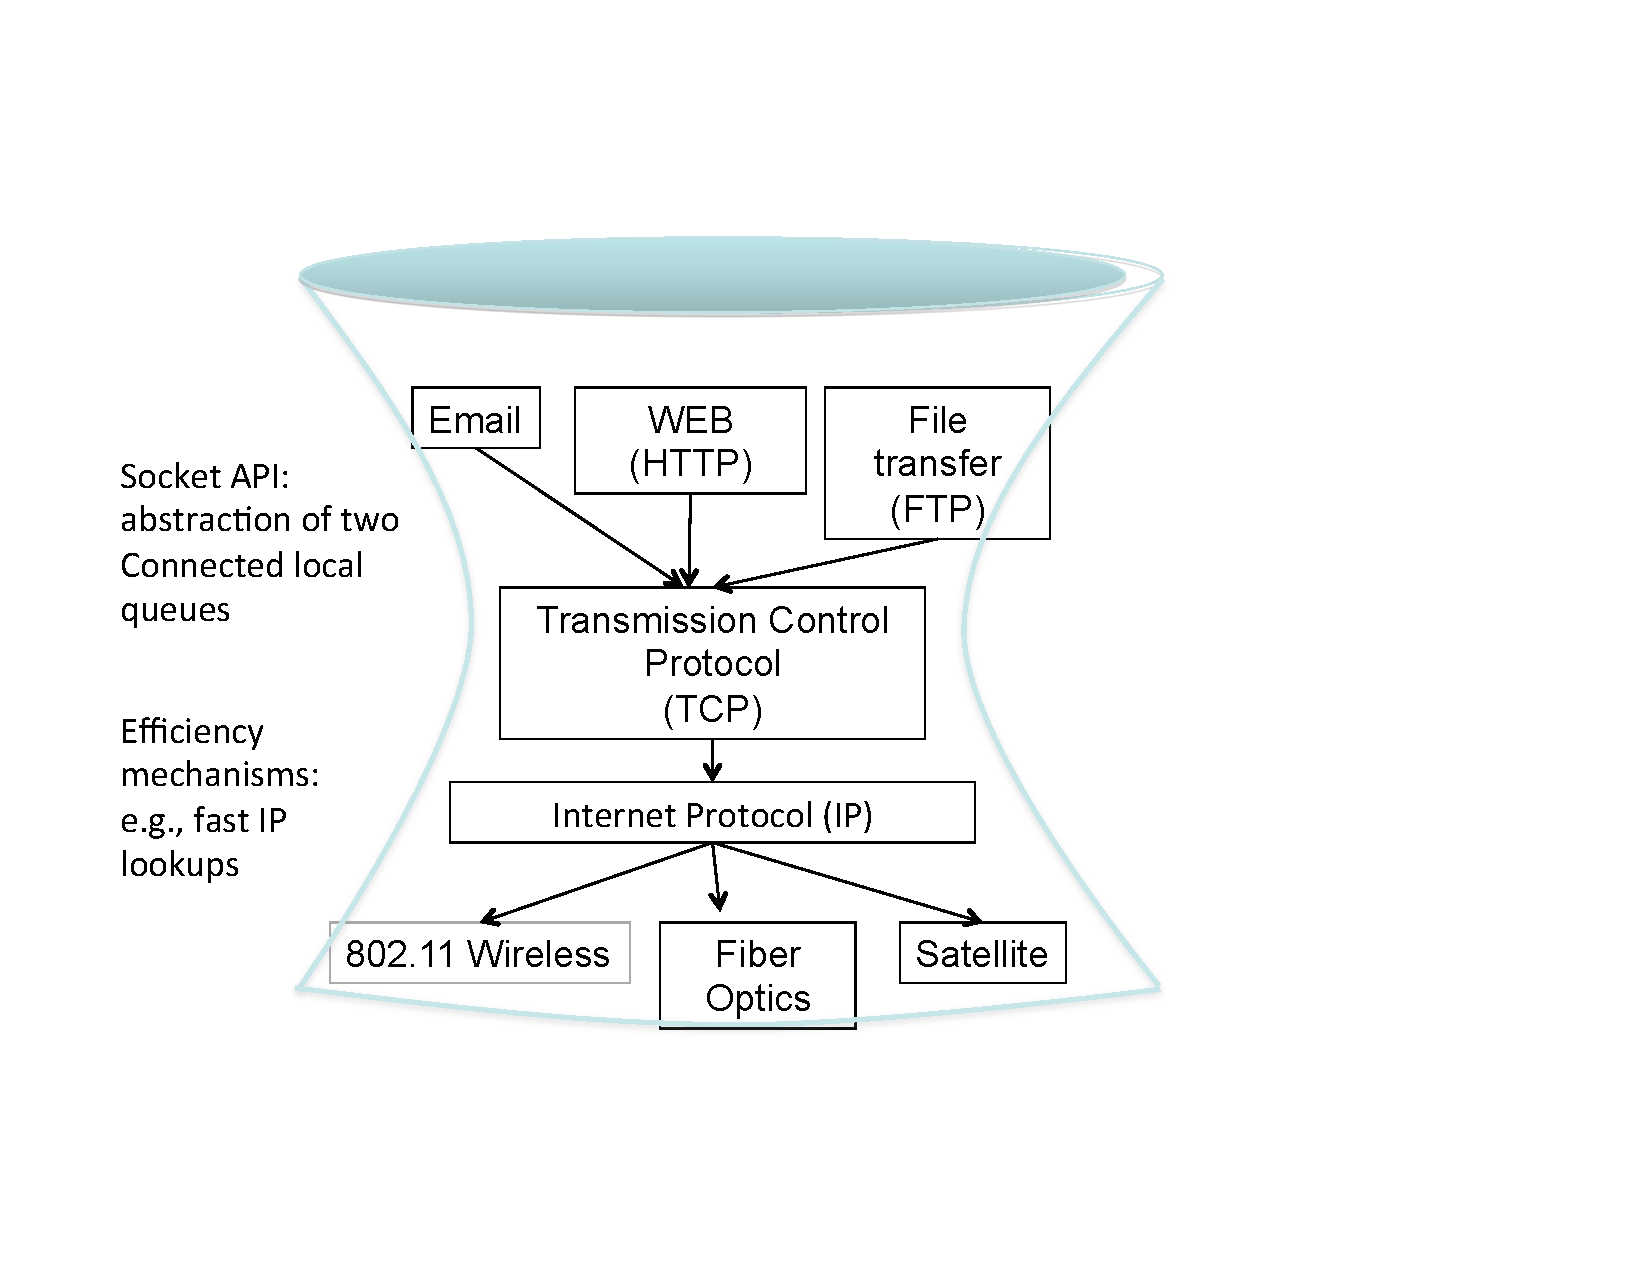
\includegraphics[trim = 0mm 40mm 60mm 10mm, clip, width=2.7in]{fig/hourglass.pdf}
  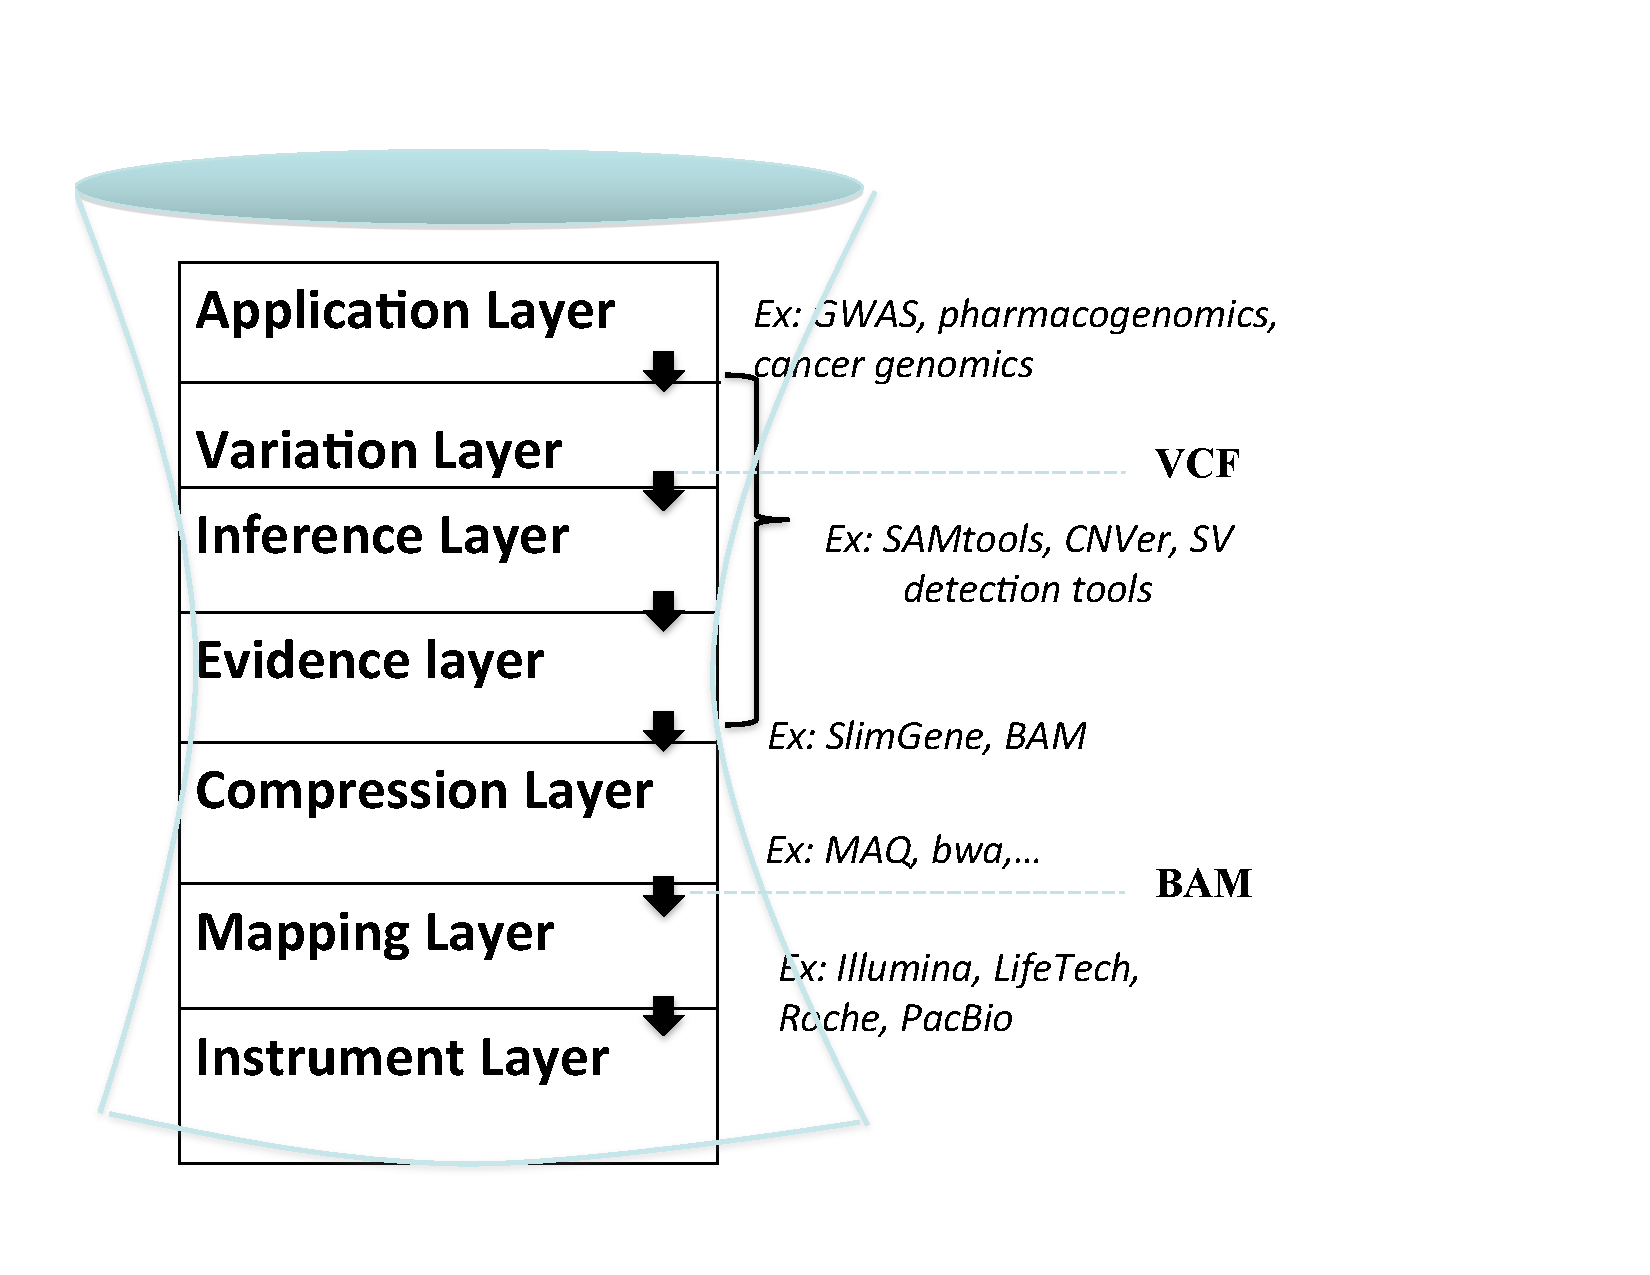
\includegraphics[trim = 0mm 15mm 40mm 10mm, clip, width=2.5in, height=1.8in]{fig/genomicabstraction.pdf}\\
 (b) 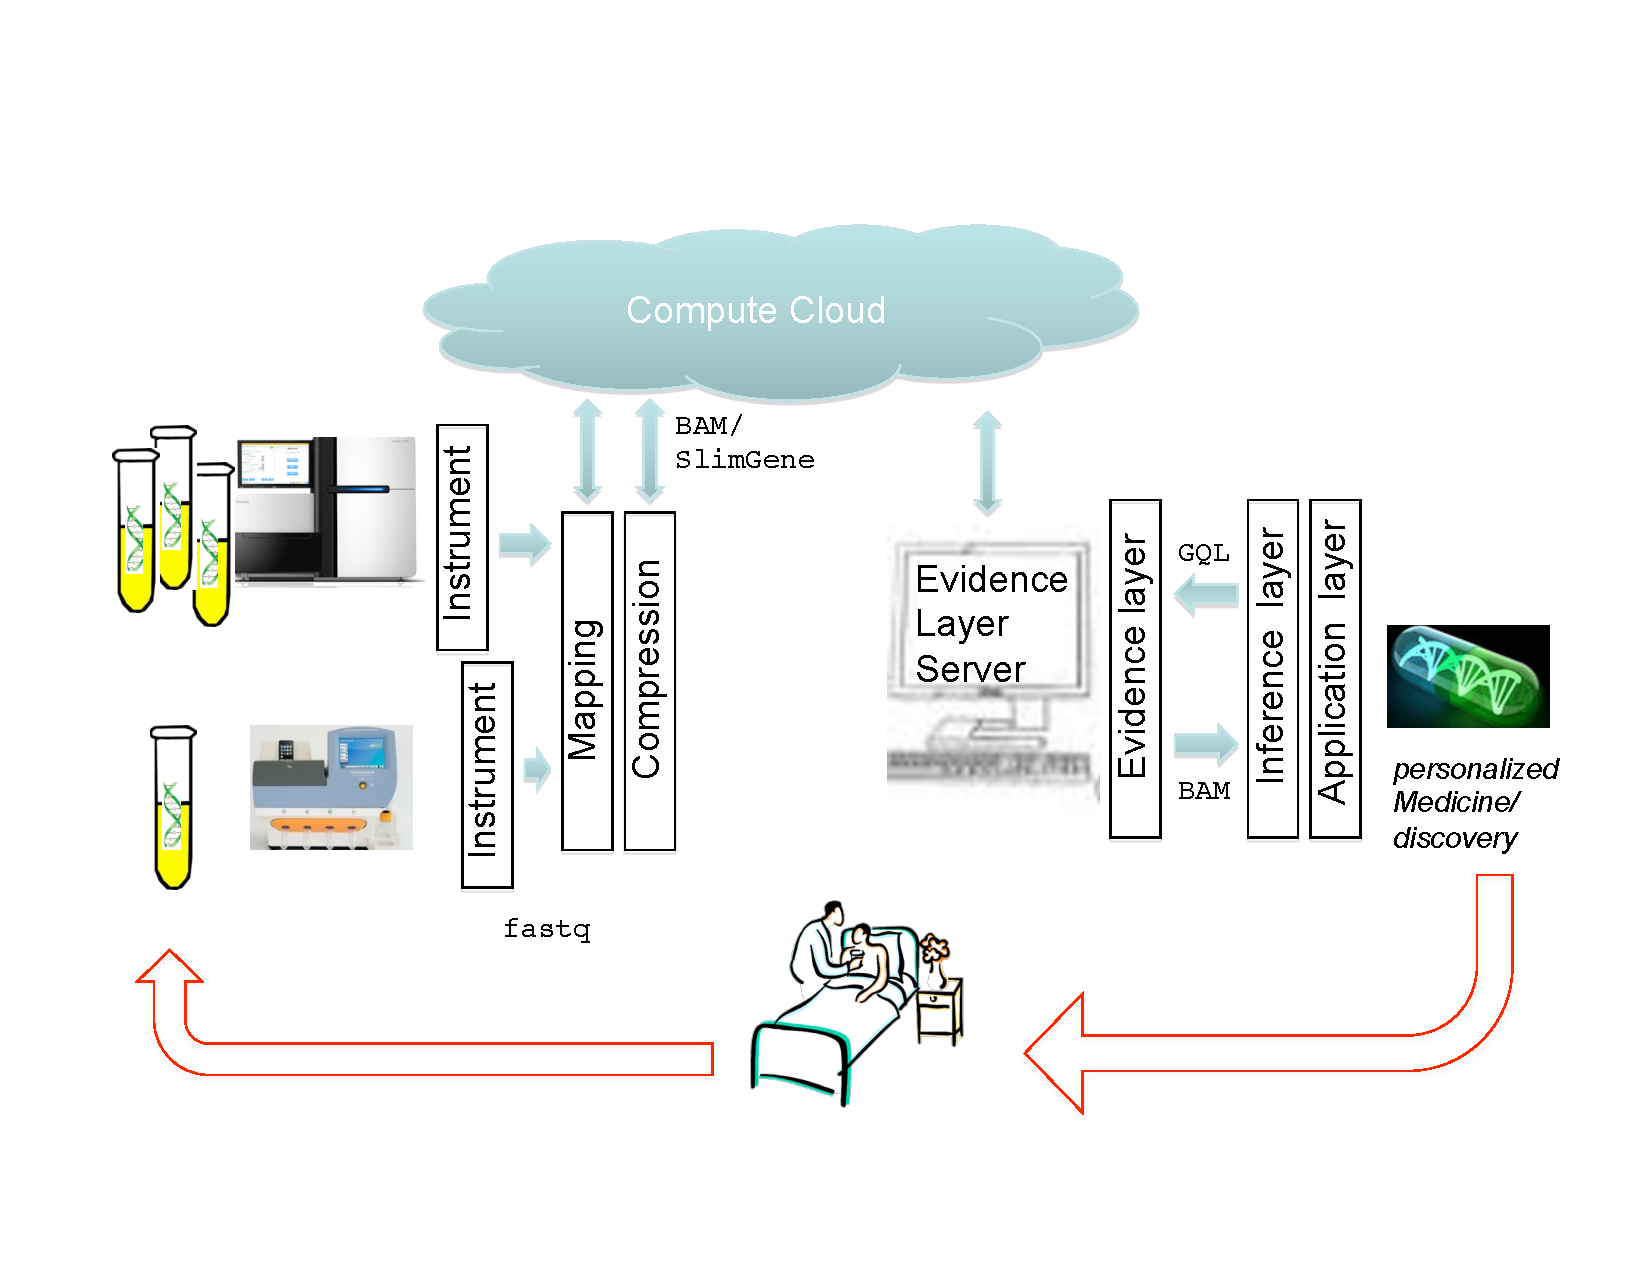
\includegraphics[trim = 20mm 20mm 10mm 30mm, clip, width=5.5in]{fig/vision.pdf}
 \caption{Abstraction for genomics. }
  \label{fig:abstraction}
\end{figure}
\subsection{The case for an evidence layer}
Recall the vision of Figure~\ref{fig:fig1}, where the genomes are produced at
different locations around the world. With redundant coverage, and
quality values, each genome is several hundred gigabytes of data. To
realize the vision of Figure~\ref{fig:fig1}, an individual laboratory needs to
process this genomic information to reveal variations and correlate
them with medical outcomes/phenotypes at each place a discovery study
or personalized medicine assay is undertaken. The obvious alternatives
are not workable, as described below.

\paragraph{Downloading raw data: } We could gather all genomic reads
subset from their distant locations on demand. However, transporting
hundreds of giabytes for each of thousands of genomes across the
network is infeasible today. Transporting disks on demand will greatly
hinder the effectiveness of such studies, especially if small changes
are required.  Compression can mitigate, but not completely avoid this
problem; our earlier results such as SlimGene show factors of 5
improvement if quality values are downloaded as well. Finally, the
processing of this data requires massive computational infrastructure,
which must be now replicated at every study location.

\paragraph{Downloading variation information:} Alternatively, the
genomic repositories could run standard variant calling
pipelines~\cite{sambam,GATK} and produce lists of variations in some
standard format such as VCF. The variant files are typically much
smaller and easier to gather on demand. Some form of relational
database may still be needed to select based on desired genetic
variations and phenotypes but the database would only stores variant
information, and therefore, could be maintained in real time across
the network.  Unfortunately, variant calling is still an inexact
science; researchers often want to use their own callers and almost
always want to see the ``evidence'' for specific variants. Even the
simplest SNV/SNP calls are an area of intense research with various
callers differing on how they rank and pool multiple lines of evidence
such as alignment quality, base pair quality values, sequencing
instrument etc.  We see no sign that this will change in the near
future or that other forms of variation will be discovered. Moreover,
the entire spectrum of variations is not well understood, especially,
large structural variations that change the architecture of the
genome. In fact researchers have called for `crowd-sourcing'
approaches to mine genomic data, with greater emphasis on discovering
novel forms of variations~\cite{Patterson2011}.

Our approach provides a desirable compromise. We \emph{allow the
  retrieval of evidence for variations on demand using a guery
  language}. The query server itself will utilize a large compute
resource like Amazon Web Services. All genomes would be accessible
(via a one-time transfer) to the server. The central server now
exports a query interface that can return the subset of reads (the
\emph{evidence}) that support specific variations, providing a higher
level interface than the first approach but lower level of access
compared to the second approach.  Indeed, some recent approaches have
hinted at this evidence layer, including SRA and
Samtools~\cite{SRA,sambam}. However, the mechanism implemented by them
(vertical slicing) involves the pre-indexing of a population of
genomic reads based on location, and mainly supports SNV/SNP calling.
However, the real power of this approach comes from making the query
language sufficiently efficient and general, that it can support the
multitude of \emph{inference engines} that do the hard work of
inferring variation using subsets of the data provided by the query
server. That is the goal of our query language. As we show below, this
approach supports multiple types of inferences, including changing
definitions of variation, and pooling of evidence across different
instrument types.

Consider a complex biological query: `` identify all deletions that
disrupt genes in a certain biological network, and the frequency of
those deletions in a natural population''.  The bioinformatician
struggles to transfer this question into a problem of statistical
inference with bounds on false-positive and false-negative
errors. However, the first part of any such query is the gathering of
the evidence. Here, the evidence would consist of all reads, and their
mappings that satisfy certain properties. For example, the reads must
overlap regions encoding genes in the given biological network, and
must fall in one of three categories: (a) Concordantly mapping reads
as these reads suggest heterozygosity of the deletion; (b) discordant
reads: all reads where the read and its pair map to locations much
further apart than could be explained by natural variation in insert
length, indicating a deletion in the donor; (c) reads in which only
one of the two ends are mapped, and which are proximal to discordant
reads, corresponding to reads that map at the boundary of the deletion
breakpoint. The development of an EL to support such queries provides
several advantages.

\begin{packed_itemize}

\item The separation allows Inference Layer designers to start
  thinking of alternate forms of evidence to improve the confidence of
  their queries.  For example, we might consider looking for
  "partially mapped" READs.  If one pair of READs overlaps the
  boundary of a deletion, then that READ will match a prefix or suffix
  of the reference and the other may match perfectly.  If the mapping
  shows that one maps correctly and the second does not, it provides
  some evidence as to the location of the boundary; further a small
  amount of effort can be used to decide if the non-mapped pair has a
  partial match with the reference.

\item The EL often poses a `data bottleneck' as it involves sifting
  through large sets of genomic reads. By contrast, the inference
  layer may be compute intensive, but typically works on smaller
  amounts of data (filtered by the evidence layer). We can implement
  EL on the cloud while the Inference Layer can be implemented either
  on the cloud or on client workstations. The evidence can easily be
  transported across the network interactively (Mbytes versus
  Gbytes). We have already seen moves by commercial cloud operators
  like Amazon to host the 1000 genome data sets on their
  infrastructure.  The cloud allows rented computation on demand
  without the cost of maintaining a permanent cluster by every
  genomics researcher.

\item The standardization of the EL will allow vendors time to
  creating a fast and scalable EL implementation.  It is hard to do
  with the Inference Layer today as it is a moving target.
\end{packed_itemize}
In the following, we develop this intuitive idea further by describing a Genome
Query Language to support the Evidence Layer.

\section{GQL: a relational language for genome queries}
\label{sec:gqa}
\newcommand{\attr}{\ensuremath{\mathit{attr}}}
\newcommand{\ID}{\ensuremath{\mathit{ID}}}
\newcommand{\GrpBy}[2]{\ensuremath{_{#1}\Gamma_{#2}}}
\newcommand{\alin}[1]{{\small\bf [[[{#1} --alin]]]}}

We want a query language that is: `complete' (i.e., capable of
handling all evidence level queries)., efficient (The query language
must have an efficient implementation), easy to express and using
standard I/O.  Ideally, it should select from a reads and output a
subset of reads in a standard format, like BAM.  We propose using a
standard SQL like syntax (SELECT from READS WHERE condition)
which will be simple and easy to use and familiar for most
programmers.  However, we argue that using a standard relational
database does not work well.

We have two fundamental types of relations.  The first are
\emph{Reads} mapped to the human genome often expressed as BAM files.
Second, we have tables of intervals representing `interesting'
(functional) regions of the genome.  While simple selection queries
are exactly as in relational languages (Select From Reads Where mapped
pairs are far apart), many useful queries require a form of joining of
relations using interval intersection and not equality as the join
operator.  For example (also see Figure~\ref{fig:mapjoin}), one might
want to join a relation consisting of READS that map to exons in a
specific gene, but where the paired-ends are far apart (indicating a
deleted exon).  We define a special \emph{MapJoin} operator to allow
this. We note that some of the newer technologies allow for multiple
reads to be generated from the same physical clone. while not
explictly discussed here, the relations can easily be extended to this
case. We also find it extremely helpful to have a third operator we
call Project Interval, which computes the largest continuous interval
containing a merged representation of what may be a number of smaller
intervals. Examples of queries using these operations are described
below.
\begin{figure}[htbp]
  \centering
 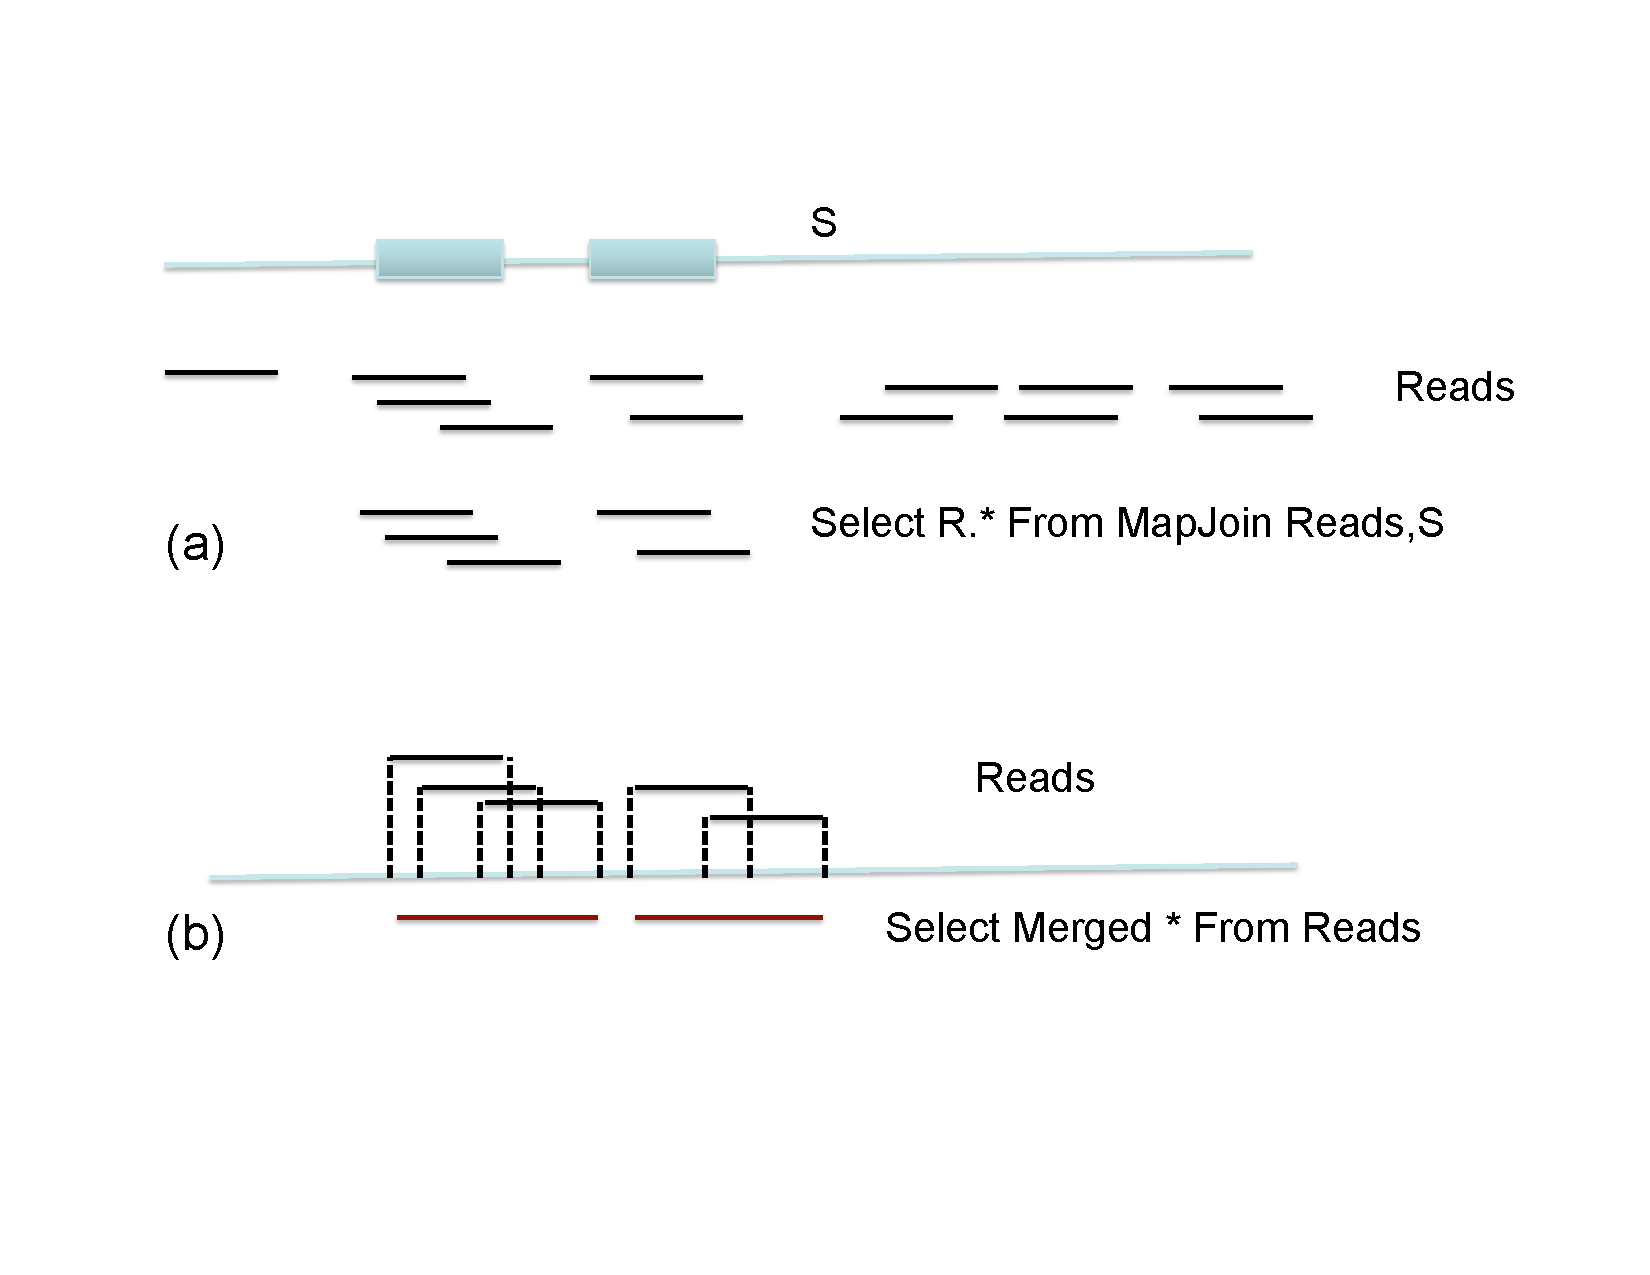
\includegraphics[trim = 20mm 50mm 10mm 10mm, clip, width=4in]{fig/MapJoin.pdf}
 \caption{Pictorial illustration of the MapJoin and ProjectInterval
   operations. (a) The MapJoin operation is a join based on intersection
   of intervals. In this figure, we project the reads that are in the
   MapJoin. (b) The Project Interval is expressed by the `Select Merged'
   command.}
  \label{fig:mapjoin}
\end{figure}
Historically, databases have been proposed for geometric queries, like
Geographics Information Sciences databases, where queries involve
joins in spatial dimensions (at least 2D while we have 1D).  While
theoretically we could coerce a GIS to do all of these things, we feel
that genomics provides a sufficiently important domain to warrant
database support from the ground up, so to speak.  We thus define a
language called GQL and show it can be used to write a number of
biologically interesting queries. The GQL is based on a \emph{Genome
  Query Algebra-GQA}, that is described in the appendix. 

As shown below, the key benefit of our proposed relational modeling is
to enable manipulation via algebraic operators (the standard
relational algebra operators, as well as domain-specific operators
defined shortly). This in turn creates the opportunity to leverage
proven techniques developed by the data management community for
efficiently querying large collections of data. Regardless of the fact
that some of these techniques need to be adapted or extended to our
specific domain, while others can be applied directly, the main
contribution here is to unlock the potential of large-scale data
processing in the context of a huge data scale challenge.

\subsection{Sample Queries} 
We have gathered many queries from practicing biologists to understand
the power of GQA. Here, we show some examples of expressive power of
the algebra. In a companion technical paper, we show that GQA's
expressive power captures the language of First Order Logic over the
relations above, as well as a signature of aggregation functions.

\begin{enumerate}

\item What is the genotype at a specific position (e.g., SNV)? 

  {\bf Query: } Let $A$ denote a relation containing the single point
  interval $\langle \mbox{chr,i,i} \rangle$. The evidence for the
  genotype at the position is provided by alignments of READS that map
  to the location, and we can either query for the mapped reads, or
  for the alignments themselves, which are often stored as a mapped
  read attribute (e.g., R.\AlignStr). Thus: \(\begin{array}{ll}
%    \mbox{GQA:} & \Project{R.ID, R.\AlignStr}(R\MapRel A).\\
    \mbox{GQL:}& \mbox{\gqlSelect\  R.ID, R.\AlignStr\  \gqlFrom\ \gqlMapjoin\ R,A}.\\
  \end{array}
  \)
\item What are the diploid haplotypes (phased genotypes; see
  Section~\ref{sec:genetics}) across a set of linked loci in a
  dataset?

{\bf Query:} This is a harder query. To assemble haplotypes we need a
collection of reads each of which (perhaps along with their paired-end
reads) connect at least two polymorphic sites.  Let attribute
$R.\mbox{CloneId}$ denote the clone identifier so that the paired-end
reads $r_1,r_2$ derived from the same clone satisfy
$r_1.\mbox{CloneId}=r_2.\mbox{CloneId}$. Also, let relation $S$ denote
the collection of point intervals, one for each variant
locus.

\begin{packed_enum}
%\item Find reads and sites they map to:  
%$$RS \leftarrow R \MapRel S$$
%\item Find reads and sites {\em their partners} map to: 
%$$PS \leftarrow \Project{\attr(R)\cup\attr(S)}(\Select{\Partner(R.\ID)=P.\ID}(R \times (\rho_P(R) \MapRel S)))$$ 

\item Find a subset of READS mapping to the loci, and the count of sites the reads or their paired-ends map to (call this count $c$):\\
  \(
\begin{array}{ll}
% \mbox{GQA:}& RC \leftarrow \GrpBy{R.CloneId}{c:count()}(R\MapRel S)\\
 \mbox{GQL:}& RC = \mbox{\gqlSelect\ } R.CloneId, c=\gqlCount(*) \mbox{ \gqlFrom\ \gqlMapjoin\ }R, S\\
&\hspace{0.2in} \mbox{ \gqlGroupby\ } R.CloneID\\
\end{array}
\)
\item Return \ID s of only those reads whose count is at least 2:\\
\(
\begin{array}{ll}
% \mbox{GQA:} &\Project{\ID}(\Select{c \geq 2}(RC))\\ 
 \mbox{GQL:} & \mbox{\gqlSelect\ } R.ID \mbox{ \gqlFrom\ }R, RC\\
 &\hspace{0.2in} \mbox{ \gqlWhere\ } R.CloneID= RC.CloneID\\
 &\hspace{0.2in} \mbox{ \gqlAnd\ } (RC.c\ge 2)
\end{array}
\)
\end{packed_enum}


\item What genomic loci are affected by Copy Number Variations (CNVs)?

  {\bf Query:} If the number of donor reads mapping to a region
  exceeds some threshold $T$ then the inference might be that the
  region has been duplicated in the donor genome. Such CNVs have been
  implicated as an important variation for many disease phenotypes. To
  gather evidence, we would like all of the intervals where the number
  of mapped reads exceeds threshold $t$ (for example). Let $G.loc$
  denote a specific chromosome and location.
  \begin{packed_enum}
  \item Compute for each location, the number of reads that map to the location:\\
    \(
    \begin{array}{ll} 
%      \mbox{GQA:} & V \leftarrow \GrpBy{G.loc}{c:count()}(R \MapRel G)\\
      \mbox{GQL:} &V = \mbox{\gqlSelect\ } G.loc, c=\mbox{\gqlCount(*) \gqlFrom\ \gqlMapjoin\ } R, G\\
      &\hspace{0.2in}\mbox{\gqlGroupby\ } G.loc
    \end{array}
    \)
  \item Return all `merged regions' where the read count exceeds threshold $t$.\\
    \(
    \begin{array}{ll}
%      \mbox{GQA:} & \ProjectInterval{G.loc} (\Select{c\ge t}(V))\\
      \mbox{GQL:} & \mbox{\gqlProjectInterval\ RS.loc} \mbox{ \gqlFrom\ } V\\
      & \hspace{0.2in} \mbox{\gqlWhere\ } V.c>t
    \end{array}
    \)
  \end{packed_enum}
    

\item Identify all regions in the donor genome with large deletions.

  {\bf Query:} As discussed earlier, the evidence for deletion comes
  from a variety of sources. We use \emph{discrepant} paired-end
  mapping. Paired-end reads from clones of length $500$ (for example)
  should map $\simeq 500$bp apart on the reference genome. If instead,
  the ends happen to map \emph{discrepantly far} (e.g., $\ell$ apart
  for some $\ell>>500$, like $\ell\simeq 10000$), they support the
  case for a deletion in the donor genome. Thus, our goal is to
  identify all regions with at least $t$ discrepant paired-end reads.
  \begin{packed_enum}
  \item Use a join in which each record contains\\ the mapping locations
    of the read as well as its paired-end.\\
    \(
    \begin{array}{ll}
%      \mbox{GQA:} & H_1 \leftarrow (\Select{R.CloneID=P.CloneID}(R \times (\rho_P(R) \MapRel G)))\\
      \mbox{GQL:} &\mbox{READS already contains this join.}
    \end{array}
    \)
  \item Select records containing discrepant reads.\\
    \(
    \begin{array}{ll}
%      \mbox{GQA:} & H_2 \leftarrow \Project{R.*} \Select {|R.loc-P.loc|>10000} H_1\\
      \mbox{GQL:} &H_2= \mbox{\gqlSelect\ * \gqlFrom\ READS }\\
      & \mbox{\gqlWhere\ }abs(loc-mateloc)>10000\\
    \end{array}
    \)
  \item Select intervals containing at least $t$ discrepant reads.\\
    \(
    \begin{array}{ll}
%      \mbox{GQA:} & \ProjectInterval{G.loc}\ \Select{c>t}\ (\GrpBy{G.loc}{c:count()}\ (H_2 \MapRel G))\\
      \mbox{GQL:} & \mbox{\gqlProjectInterval\ G.loc \gqlFrom\ } H_2\\
      & \mbox{\gqlGroupby\ G.loc, c=count(*)}\\
      & \mbox{\gqlWhere\ } c>t\\
    \end{array}
    \)

  \end{packed_enum}

\end{enumerate}


\subsection{Population based queries}

The true power of querying genomes comes from the ability to query
populations. Indeed, existing tools (Samtools) allow for the ability
to extract reads from multiple individuals at specific locations
corresponding to polymorphic sites. We want to extend the full power
of genomic queries to interrogate populations. Recalling the warfarin
example, we would like to query for warfarin dosage and genetic
variation in candidate genes (genes identified through a discovery work
flow) among individuals on the warfarin regimen. Specifically, we
could be interested in copy number changes.

\noindent \emph{{\bf Colloquial:} Report warfarin dosage and genomic
  intervals in individuals s.t. (i) the individuals are on the
  warfarin regimen, and (ii) the genomic intervals intersect with some
  gene in a candidate set $E$, and (iii) the copy number of mapped
  reads is at least twice the expected coverage in the interval}

Consider a population relation $P$ of individuals that have been
sequenced. Individuals in the population have `phenotype'
attributes. The attributes could be, for example, diseases, treatment
regimen (``P.W'' is set for individuals taking warfarin), and could be
categorical, or continuous valued (``P.WD'' for warfarin dosage). The
natural join $P\NatJoin R$ describes relations $(p,r)$ in which
attributes of read $r$ are linked to the attributes of individual
$p$. To answer the query, first we identify all reads that map to gene
intervals $E$, and are sampled from individuals on warfarin
regimen. For example,

    \(
    \begin{array}{ll}
      \mbox{GQL:} &\mbox{\gqlSelect\ * \gqlFrom\ P,\gqlMapjoin R,E }\\
      & \mbox{\gqlWhere\ P.WD = TRUE}\\
    \end{array}
    \)
%\[
%W' \leftarrow  \GrpBy{E.loc}{c:count(R.ID)} (W)
%\]

Next, count the number of reads at each location. Finally, we project the locations and reads where the coverage is higher than threshold $T$.
%\[
%    \Project{E.loc, R.ID}\:\:\Select{c \ge T} (W')
%\]
A similar idea applies to a \emph{personalized workflow}, where we
ask: \emph{report warfarin dosage in individuals with copy numbers
  matching the query individual $p$ at the candidate set $E$ }.

To gather evidence, we collect the set of reads and their copy numbers
mapping to $E$ in all individuals on a warfarin regimen. From this
set, we select the individuals and READS whose copy counts `match up'
with $p$

%Thus, we have
%\[
%W\leftarrow \GrpBy{E.loc}{c:count(R.ID)} (W) \Select{{\scriptsize \mbox{P.W}}} (P\NatJoin R\MapRel E)
%\]

%\[
%\Select{P.c\simeq p.c } W
%\] 

{\bf Group Inference without Accurate Individual Inference:} The
ability to query populations has an important benefit. For individual
genomes, calling SNVs accurately is often challenging. The Inference
layer assigns quality values to individual SNV calls (e.g., SNV at Chr
10:10500 with probability 0.8), and these confidence values are used
for association with phenotypes in a segregating population.  By
contrast, population queries allow us to ask for evidence about
arbitrary subsets of large groups of users based on various
characteristics of these users and doing statistical inference
directly on these large groups. They allow us to bypass the
determination of individual SNVs. Often, individual SNVs may have very
little evidence for low-coverage sequencing. However, if a large
number of affected individuals in a population (e.g., 800 out of 1000)
all show the same SNV, while controls do not, we can reliably predict
an association even with unreliable calls for individuals.  While more
work is required to demonstrate the benefits of group inference, the
important point is GQL provides query support for group inference.

\section{A prototype implementation}
We have developed a prototype implementation, \emph{genomequery} of a
subset of GQL (Figure~\ref{fig:genomequery}), with visualization
provided by the open-source tool jbrowse~\cite{Skinner2009}. The
uploaded genome (in BAM format) can be queried using a simple text
interface that allows the user to write a GQL query. The query is
compiled and executed, and the output returned as a (smaller) BAM file
that can be visualized using jbrowse, or downloaded to the client for
further analysis.

\begin{figure}[ht]
  \centering
  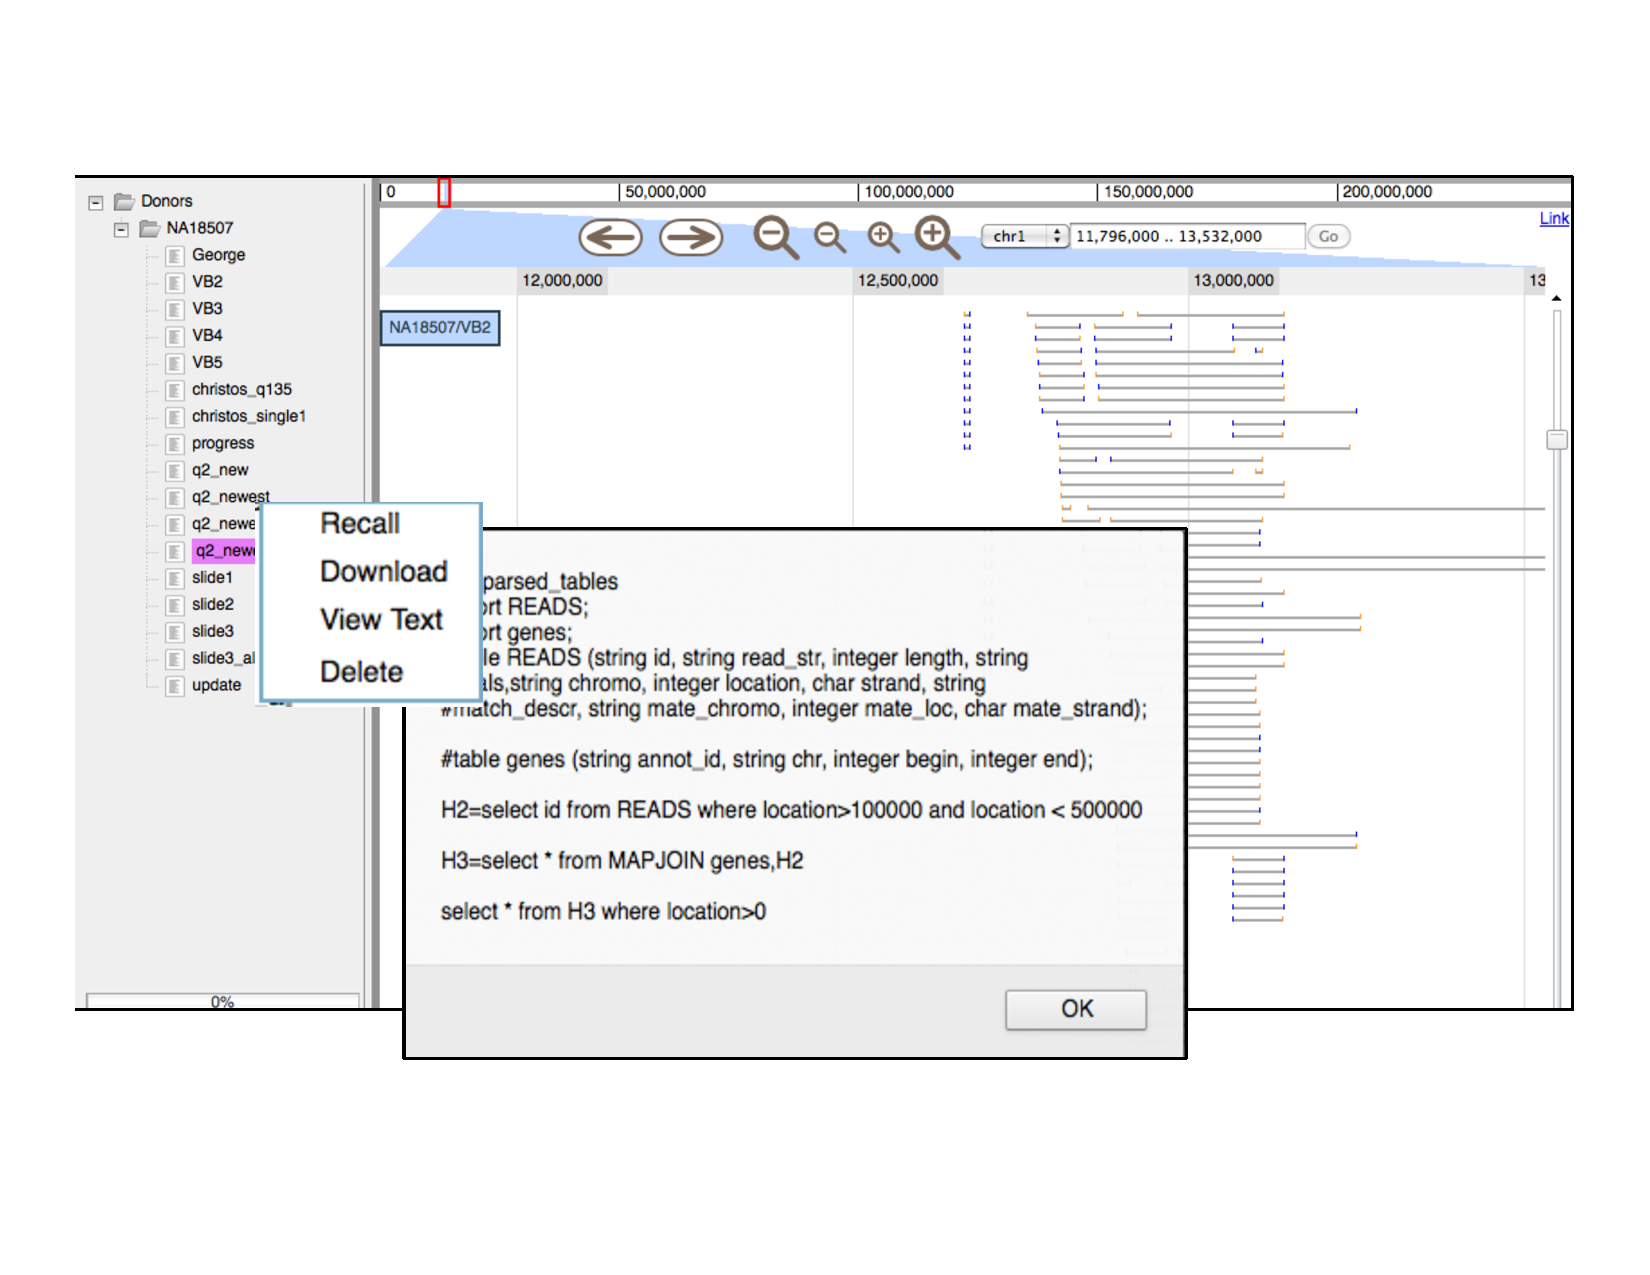
\includegraphics[trim = 10mm 35mm 10mm 25mm, clip,width=4.5in]{fig/genomequery.pdf}
  \caption{A prototype implementation of GQL, with visualization using
    the open source tool jbrowse~\cite{Skinner2009}. Discordant
    paired-end reads supporting deletions can be seen.}
  \label{fig:genomequery}
\end{figure}
The implementation of \emph{genomequery} has a customized parser that
converts GQL to an intermediate representation resembling GQA. Thus,
there are customized procedures for each of the algebraic operations,
with some concessions for efficiency (mainly w.r.t
memory). Specifically, we use interval trees to implement $\MapRel$,
and customized indices (including Strength Vectors; see below) for
efficient querying. Details on the implementation will be provided
elsewhere. 

\section{The way forward: challenges for computer scientists}
\label{sec:futuredirections}
At this point, we have made the case for a set of genomic layers,
including an Evidence Layer where the genomic evidence is retrieved
using a Genome Query Language. Successful implementation of this
vision will depend upon some new ideas from computer science: the
specific areas are marked in the subsection titles

\subsection{Scope of querying -- Database Theory}
On the language design front, we ask if the Genome Query Language
(calculus) GQL and the Genome Query Algebra GQA are sufficiently
powerful to address all Evidence Layer queries needed in practice to
truly support the inference layer.  The goal is to push into the
Evidence Layer as much of the data-intensive computation as possible
while preserving performance (note that, absent this desideratum, any
query language that can return a copy of the relations provides
trivial support by relegating the entire computation to the inference
layer). Our design has been guided so far by the relational gold
standard. That is, GQL and GQA have identical expressive power, which
coincides with that of first order logic over the schema of the three
relations $R,G,P$, a signature of aggregation functions, and a
group-by operator.  As an immediate consequence, this allows the usage
of GQL as a highly declarative language for application developers,
and the deployment of GQA as the internal representation used to
optimize and evaluate query plans. Relational experience suggests that
special-purpose indexes and optimization will play a crucial role in
pursuing this goal.

Our preliminary study of high-frequency analysis tasks has yielded a
query exemplar that is covered by the expressive power built into the
first-cut language draft. Further user feedback may require
extensions. In implementing them, care must be taken to balance
expressive power with efficient evaluation.

\subsection{Efficient querying --- Database Implementation}
As a first step assume that queries on populations will automatically
be decomposed into queries on individuals. Consider queries of the
general form \gqlSelect $\:a\:$ \gqlFrom $\:$ \gqlMapjoin $\:R,G\:$ \gqlWhere $\:b$. The two
steps are
%\begin{enumerate}
\begin{packed_enum}
\item Select for relations that satisfy constraints $b$.
\item Project (while removing duplicates) on to attributes $a$.
\end{packed_enum}
%\end{enumerate}
We present some straightforward indices that help speed up
computations. Consider an index {\sc LocationToReads}, where {\sc
  LocationToReads}$(\ell)$ is a pointer to first read $r$ that maps to
the point-interval $l$. For each individual, we keep a compressed
index of the mapped reads in memory. The index can be used for Select
operations based on specific locations (e.g, reads that map to
specific genes).

However many queries involve scanning the entire genome for maximal
intervals. For example, find all maximal regions where there is a
disproportionate increase in the number of mapped reads (High copy
number). 

%The corresponding GQA is given by
%\begin{eqnarray*}
%  \ProjectInterval{G.loc}\:\:\Select{c \ge t} \GrpBy{G.loc}{c:count(R.ID)}  (R\MapRel G)
%\end{eqnarray*}
%Generalizing, we may have other constraints encoded by $\theta$, and
%consider queries of the form
%\begin{eqnarray*}
%  \ProjectInterval{G.loc}\:\:\Select{c \ge t} \GrpBy{G.loc}{c:count(R.ID)} \Select{\theta} (R\MapRel G)
%\end{eqnarray*}

For efficient implementation of these queries, we construct special
indices that allow filtering for READS according to a user-defined
constraint. Define an attribute {\em strength vectors} $S_{\theta}$ for a
constraint $\theta$ as a vector of length $G$ (the entire genome).
%\[S_{\theta} \leftarrow \Project{G.loc,c.count}\:\: \GrpBy{G.loc}{c:count(R.ID)} \Select{\theta} (R\MapRel G)
%=\]
Thus for any location $\ell \in G$, $S_{\theta}[\ell]$ gives the
strength of the evidence at that location, and can be precomputed for
common constraints $\theta$. Clearly, the strength-vectors allows us
to efficiently search for intervals with high strength. Strength
vectors are memory intensive. To get around that, we choose a minimum
cut-off such that only intervals above the cut-off are
interesting. Define a compressed strength vector $C_{\theta,t}$ as a
sorted sequence of intervals $i_1, i_2, \ldots$ such that each $i_j$
is a maximal interval satisfying $S_{\theta}[\ell] \geq t$ for all
$\ell\in i_j$.  In other words, we only store the subintervals of the
genome where the strength for the predicate is sufficiently high.  Of
course, if the user changes the threshold $t$ to a lower value, the
strength vectors have to recomputed using {\sc LocationToReads}.

If the compressed strength vector is $100\times$ smaller than the
strength vector, it will be correspondingly faster to read it off
disk.  For large populations, where the compressed strength vectors
must be loaded off the disk iteratively, this offers a great speed
advantage. The trick is to choose thresholds appropriately so that the
inference layer can get a superset of what it needs, but that is still
smaller than the set of all READS. 

\old{
Consider the query from before
\[
   \Project{g}\:\: \Select{{\scriptsize \mbox{p.d {\sc and} HighCNV}(R,g)}} (P\NatJoin R\MapRel G)
\]
We use the natural join $P\NatJoin R$ select all records corresponding
to individuals satisfying ``p.d'' and project out the corresponding
pointers to their compressed strength vectors. We now traverse each
compressed strength vector, incrementing the count for each location
spanned by subinterval $i$ of the compressed strength vector for
patient $j$.  We keep track in an output queue of all locations whose
counts are over some threshold $r$.  It should be clear that this can
be generalized to more sophisticated queries (e.g., locations in which
$X\%$ of patients have high copy number and$Y\%$ of non-patients have
low copy number). 
}

\subsection{Interface with Electronic Medical Records -- Information Retrieval}
We have so far glossed over the effort required to record phenotypes
associated with each sequenced individual: a list of diagnoses (e.g.,
diabetes Type 1), clinical findings (e.g., elevated HbA1C), and
therapies (e.g., insulin), as well as demographics (e.g., age and
gender). Such information is already in patient medical
records. Initial results from the eMERGE network indicate that, for a
limited set of diseases, it is possible to utilize the EMR for
phenotype characterization in genome wide association studies (GWAS)
within a reasonable margin of error\ncite{Kho2011,Pathak2011}. It is
anticipated that most healthcare institutions will be utilizing EMRs
by 2014, given incentives provided by the HITECH act\ncite{Stark2010},
and it is also expected that more genome information will become part
of the EMR, well beyond the cursory data on select SNPs that is
available from GWAS. This will require significant modification of EMR
systems so that the personal genome information can be utilized in
real-time, at the point of care. Given the increasing adherence to
standards for interoperability in clinical documents\ncite{Dolin2011}
and important advances in biomedical natural language
processing\ncite{Nadkarni2011}, a large portion of the EMR is now
structured in a way that all data from a given patient can be
retrieved efficiently.  However, there is essentially no effective
integration of genotype and phenotype data, hence there is significant
work remaining that is related to software engineering. Furthermore,
several issues related to querying across a group of patients need to
be addressed. Although high level abstractions of the information
obtained from genome sequences are already part of the EMR as
laboratory tests (e.g., specific SNPs in BRCA1 or 2), systems that
allow whole genome sequences to be queried in real-time to assist in
clinical decision making are yet to be developed. Furthermore, GQL
should be useful both for interrogating a single genome or
interrogating several genomes across groups of individuals. Most EMR
systems in the market today are based on hierarchical databases
optimized to retrieve all data from a single patient. Significant
transformations of transaction-based EMRs are needed to allow
efficient queries on multiple patient records. For example, relational
databases are implemented to allow efficient queries for populations,
constituting the basis for clinical data warehouse
systems\ncite{Chute2010}. GQL should integrate with these systems so
that EMR data could be queried together with genome data.


\subsection{Privacy concerns -- Computer Security}
The genome is the ultimate unique identifier. All privacy is lost once
we have access to the genome of an indvidual, but the current
regulation, the Health Information Portability and Accountability Act
(HIPAA) is silent about this
identifier\ncite{Annas2003,Benitez2010,Malin2011}. Although the Genetic
Information Nondiscriminating Act (GINA) addresses accountability for
use of genetic information\cite{Hudson2008}, privacy laws will need to
change to ensure that sensitive information is available only to the
appropriate person. Regardless of what the privacy laws are/will be,
they all hinge on some definition of which information about an
individual is ``leaked'' when some study results are
disclosed. Checking that a given study satisfies a specific privacy
definition requires formal reasoning about the data manipulations that
generated the disclosed data, which is impossible without a
declarative specification of such manipulations, with rigorous
semantics. This is exactly what GQA queries offer. Of course, an
equally rigorous semantics for privacy, adopted legally, is required
to complete the picture. Current efforts involve the investigation of
differential privacy\ncite{Chaudhuri2011}, as well as multiple types
of de-identification
procedures\ncite{OhnoMachado2004,OhnoMachado2011}. While this is not
within the scope of this article, GQA at least enables a design
process to start. Typically, such a design process for privacy
measures tries to maximize the class of allowable study outputs.


\subsection{Provenance -- Software Engineering}
GQL is an ideal vehicle for recording provenance of study conclusions,
by recording the set of queries launched for a specific study.  The
declarative nature of such queries renders them orders of magnitude
more readable by humans and programs than the scripts used currently
to code the data manipulations. Such scripts are usually not
publishable, because they consist of code that is often too ad-hoc for
human readability, and because they span various programming
languages, which are often too rich and low-level for automatic
analysis.  Publishing the set of queries along with their results
would significantly enhance the clarity of the study's claims, as well
as its repeatability.

A further benefit of storing study result provenance as queries is to
pave the way for tools that react automatically when the input data to
the study changes (an all too common event).  This happens when the
input data producer (possibly a set of autonomous third-party labs),
adds new data entries, or retracts or corrects old ones.  By analyzing
the query expressions, changes to the study's input data can be
automatically propagated to the output in an incremental fashion,
without re-running the entire expensive query from scratch.  The
relational analogy to this scenario is known in the database literature
as 'incremental view updating', and is being used successfully in data
warehousing applications.
 
Finally, the practice of disclosing provenance queries along with each
study result would enable scientists to reuse the data of previously
published computing-intensive studies. Instead of running her
expensive queries directly on the original input databases, the
investigator would launch an automatic search for previously published
studies whose provenance queries correspond to (parts of) the
computation needed by her own queries.  The results of the provenance
queries can be directly imported and used as partial results of the
new study's queries, skipping re-computation.  This scenario
corresponds in relational database practice to that of 'rewriting
queries using views'. Views are cached results of previously executed
queries, each result annotated with the actual query expression.  In
essence, rewriting algorithms try to match query and view expressions
against each other to determine reusability, thus relying crucially on
the availability of the query expressions.

\subsection{Inference at Scale --- Learning Theory, Probabilistic Inference}
We have suggested that learning the correlation between diseases and variations
can be tackled differently if there are a large number of genomes.  Perhaps, 
it is less critical to evaluate individual variations for such a discovery problem,
because erroneous variations are unlikely to occur over a large group of randomly
chosen individuals.   More generally, what other inference techniques are there that
leverage the presence of data at scale.   For example, Google leverages the large
data it has to find common misspellings.   Note that carefully screening individual
variations is still needed for personalized medicine. 

\subsection{Crowd-sourcing}
An intriguing suggestion from Patterson is the use of crowd-sourcing
techniques to solve hard challenges like
cancer\cite{Patterson2011}. To enable this, the query system must have
the mechanisms to allow a group to work coherently on the problem.
For example, consider the scenario where talented high school science
students look for genetic associations using genomes from cases and
controls for specific diseases. A mechanism that could be useful is
the selection of a \emph{random} subset of cases and controls, which
are nevertheless genetically matched (arising from a single, mixing
population). Then, instead of selecting from all (tens of thousands of)
individuals, one could query for a random subset of $100$ individuals
using a fraction of network bandwidth, while still providing similar
statistical power for detecting associations.


\subsection{Commoditizing Genomics -- Computer Systems}

Genomics and personalized medicine must be commoditized to be
successful.  Such commoditization requires computer system research.
For example, Amazon has already moved a number of genomes in the 1000
genomes project where they are accessible via S3 storage.  However,
the amount of data is so vast that manipulation and visualization over
the cloud is still expensive and time consuming.  We see several
avenues for improvement.  First, since most genomes are read only, it
makes sense to leverage new technologies such as solid-state disks
(SSDs).  Second, efficient decomposition between the cloud and the
workstation will be key to reducing data traffic in and out of the
cloud, a major bottleneck today.  Our layering suggests that the
Evidence Layer be deployed in the cloud and be accessible via GQL, and
the results be visualized or inferenced in a workstation.  Much clever
decompositions are clearly possible.  Third, while genomics has been
dominated historically by expensive parallel computers it will be
important to tailor processing software to cheap multicore CPUs to
improve locality of reference.


\section{Conclusion}
\label{sec:conclusion}

Genomics is moving from an era of scarcity (a few genomes with
imperfect coverage) to abundance (universal sequencing with high
coverage and cheap resequencing when needed).  This shift requires
rethinking genomic processing from ad hoc tools and pipelines that
support a few scientists to commodity software that can support a
world of medicine.  The history of computer systems teaches us that as
systems move from scarcity to abundance, modularity is paramount; ad
hoc software is replaced by a set of layers with well defined
interfaces as in Operating Systems (application, kernel, drivers) and
networks (TCP, IP, Link Layers).  That these trends have been
recognized by industry can be seen by the shift from machine specific
formats such as Illumina to standards such as BAM, and from vendor
specific variant formats to VCF.  The 1000 genomes project has gained
momentum and a large number of sequences are already accessible.
However, much of the progress today has been to define data formats
without powerful interface functionality; to use an Internet analogy
this is as if TCP packet formats were defined without the socket
interface.

Our paper proposes going beyond the layering implicit in current
industry standards, and suggest that such layering can enable
personalized medicine and discovery.  Specifically, we proposed the
separation of evidence from inference, and the separation of
individual variation from variation across groups
(Figure~\ref{fig:abstraction}a)).  More concretely, we propose a
specific interface between the EL and the IL via a Genome Query
Language (GQL).  While GQL is based on a relational model using a
virtual interval relation, we have found that effort is required
beyond standard relational optimization to allow GQL to scale to large
genomes and large populations.

We described several benefits to separating evidence from inference.
A vast genome repository accessible by GQL offers the ability to reuse
genomic data across studies, the ability to logically assemble
case-control cohorts, and the ability to rapidly change queries
without time consuming ad-hoc programming.  GQL also offers the
ability to reduce the quality of inference on an individual basis when
doing group inference on large populations.

We described some simple ideas to scale GQL to populations using
compressed strength indices and doing EL processing in the cloud.
However, much work remains to be done to complete this vision
including better large scale inference, system optimizations to
increase efficiency, information retrieval to make medical records
computer readable, and security mechanisms.  While the work is vast,
so is the opportunity.  It is not often that one gets the chance to
work on a large system such as the Internet or UNIX that can change
the world.

\section{Acknowledgment}
The authors acknowledge support from the NIH sponsored iDASH project
(Grant U54 HL108460), NIH 5R01-HG004962, and a CSRO scholarship to
CK. Some of us would also like to thank Rajesh Gupta, Vish Krishnan,
Ramesh Rao, and Larry Smarr for useful discussions and support.

\bibliography{query.bib}
\newpage
\section{Appendix}

Our database has some key relations. The first is \emph{R (Reads)}
that describe the set of read fragments output by the sequencer, and
all of their properties.  For example, for paired-end sequencing, $R$
could contain identifiers for each read $r$, and its paired-end. A
second relation encodes a set of intervals on the genome, where each
is specified by the triple ``$\langle\mbox{chromosome, start-position,
  end-position} \rangle$''. A specific, and important, case of the
interval relation is the relation $G$ (the genome) where each entry is
a point interval corresponding to a specific location ({\em locus })
on the genome. As $G$ is large ($3\cdot 10^9$ loci), we do not
materialize $G$ explicitly, using it instead as a virtual (conceptual)
relation to facilitate the relational expression of queries. A final
relation $P$ describes the set of all individuals in a population, and
will be discussed in a subsequent section.



\paragraph{Standard relational algebra operators and language
  constructs}
Standard algebraic operators we use in the examples below include: 
\begin{packed_itemize}
\item The projection operator $\Project{}$ where $\Project{X}(E)$
  returns, from the relation $E$ evaluates to, the restriction of the
  tuples to the attributes named in $X$. In GQL, we express this
  operation using
  \[
  \mbox{\gqlSelect\ } \mbox{X}  \mbox{ \gqlFrom\ }  E
  \]
\item The selection operator $\Select{}$, where $\Select{\theta}(E)$
  selects the subset of precisely those tuples in the result of
  expression $E$ that satisfy filter predicate
  $\theta$. Correspondingly, in GQL:
  \[
  \mbox{\gqlSelect\ * \gqlFrom\  E \gqlWhere\ } \theta
  \]
\item The Cartesian product operator $\times$, where $E\times F$
  refers to all tuples of the form $(e,f)$ where $e\in E, f\in F$. In
  GQL:
  \[
    \mbox{\gqlSelect\ * \gqlFrom\  E,F}
  \]

\item The renaming operator $\rho_N(E)$, which sets to $N$ the name of
  the relation returned by $E$.
\item The group-by operator $\GrpBy{}{}$, where in
  $\GrpBy{G_1,G_2,\ldots,G_k}{N_1:F_1(A_1),\ldots,N_l:F_l(A_l)}(E)$,
  $E$ is an algebraic expression that evaluates to a relation,
  $G_1,\ldots,G_k$ are group-by attributes, each $F_i$ is an aggregate
  function and each $N_i,A_i$ are attribute names.  The meaning of the
  group-by operator is the standard one: all tuples in the result of
  $E$ are partitioned into groups, such that two tuples are in the
  same group if and only if they agree on the values of all group-by
  attributes.  Thus, the groups can be identified by the value of the
  group-by attributes.  For each group $(g_1,\ldots,g_k)$, the result
  contains a tuple of attributes $G_1,\ldots,G_k,N_1,\ldots,N_l$ and
  values $(g_1,\ldots,g_k,n_1,\ldots,n_l)$, respectively. Here, each
  $n_i$ is computed by applying function $F_i$ to the collection of
  attribute $A_i$'s values found in the group. In GQL:
\[
  \begin{array}{l}
    \mbox{\gqlSelect\ } G_1,\ldots,G_k,N_1=F_1(A_1),\ldots,N_l=F_l(A_l) \mbox{ \gqlFrom\ }  E\\ 
    \mbox{\gqlGroupby\ } G_1,\ldots G_k
  \end{array}
\]



By default, this
  collection is viewed as a multiset, i.e. duplicate values are not
  removed.  To apply $F_i$ after eliminating duplicates, we use the
  syntax $N_i:F_i(\mbox{distinct\ } A_i)$.  The syntax of the count
  aggregation is an exception, in that no $A_i$ attribute need be
  specified.
\end{packed_itemize}


\paragraph{The Map join and the Project Interval operator:}
As reads are sequenced, they are also mapped to the reference genome
using various mapping algorithms. Some mapping algorithms map each
read to a unique location, or not at all; others may choose to
identify all intervals where the underlying genomic string is similar
(in terms of edit distance) to the read. For now, assume that each
read is mapped to its best location by a mapping algorithm $M$, and
the relation $R$ includes the interval of the best map.
\old{ (i.e. $\ID \subseteq \attr(R)$, where $\attr(R)$ denotes the set
  of $R$'s attributes). Note that under this assumption, the \ID\
  attributes uniquely identify each read (tuple in $R$).}


For an arbitrary relation of genomic intervals, $A$, define a
\emph{map-join} operation $R\MapRel A$ by a pair of tuples $(r,g)\in
R\times A$ such that (r.chr, r.start, r.end) and (a.chr, a.start,
a.end) `intersect'. Recall that we defined the relation $G$ as the set
of all genomic loci. Therefore, $R\MapRel G$, denotes the set of all
tuples $r,g$ where $g$ denotes a genomic coordinate that $r$ maps to.
In many practical instances, the relation is quite large. If 33\% of
the genome was mapped on the average by 10 reads, $R\MapRel G$ would
contain $\simeq \frac{1}{3} 3\cdot 10^9\cdot 10= 10^{10}$ tuples. In
GQL:
\[
    \mbox{\gqlSelect\ } * \mbox{ \gqlFrom\ \gqlMapjoin\ }  R,G\\ 
\]


To reduce output size, we define a special \emph{Project-interval}
operator $\ProjectInterval{}$. $\ProjectInterval{A.ID} (R\MapRel A)$
outputs all genomic intervals after `fusing' adjacent and overlapping
intervals. Thus,
\[
\ProjectInterval{G.ID} (R\MapRel G)
\] 
would result in the set of all disjoint genomic intervals with some
read mapping to them. Correspondingly, in GQL:
\[
    \mbox{\gqlProjectInterval\ G.ID} \mbox{ \gqlFrom\ \gqlMapjoin\ }  R,G\\ 
\]

\end{document}


